\chapter{Using the WP Plug-in}
\label{wp-plugin}

The \textsf{WP} plug-in can be used from the \textsf{Frama-C} command line
or within its graphical user interface. It is a
dynamically loaded plug-in, distributed with the kernel since the
\textsf{Carbon} release of \textsf{Frama-C}.

This plug-in computes proof obligations of programs annotated with
\textsf{ACSL} annotations by \emph{weakest precondition calculus},
using a parametrized memory model to represent pointers and heap
values. The proof obligations may then be discharged by external
automated theorem provers such as
\textsf{Alt-Ergo}~\cite{AltErgo2006},
\textsf{CVC4}~\cite{CVC4} and
\textsf{Z3}~\cite{Z3}
or by interactive proof assistants
like \textsf{Coq}~\cite{Coq84} and more generally, any automated or interactive
prover supported by \textsf{Why3}~\cite{Why3}.

\clearpage
\section{Supported annotations}

The \textsf{WP} plug-in supports the following code annotations. We also
indicate the number of verification conditions that are generated in the
default configuration:
\begin{itemize}
  \item \lstinline{lemma}: 1 VC
  \item \lstinline{axiom}: no VC (admitted with no proof)
  \item \lstinline{ensures}: 1 VC
  \item \lstinline{exits}: 1 VC
  \item \lstinline{disjoint}: 1 VC
  \item \lstinline{complete}: 1 VC
  \item \lstinline{requires}: 1 VC for each call
  \item \lstinline{terminates}: 1 VC for each call, 1 VC for each loop without "loop variant"
  \item \lstinline{decreases}: 1 VC for each recursive call
  \item \lstinline{assigns}: 1 VC for each assigned lvalue
  \item \lstinline{admit}: no VC (admitted with no proof)
  \item \lstinline{assert}/\lstinline{check}: 1 VC
  \item \lstinline{loop invariant}: 2 VCs (established, preserved)
  \item \lstinline{loop variant} (integer): 2 VCs (positive, decreasing)
  \item \lstinline{loop variant} (general measure): 1 VC (the measure is \emph{assumed} to be well-founded)
  \item \lstinline{loop assigns}: 1 VC for each assigned lvalue within the loop
\end{itemize}
The statement contracts are not supported. The number of generated verification
conditions can vary depending on the selected options. See for example the
options listed in~\ref{subsec:computation-strategy}.

In addition, the \textsf{WP} plug-in asks the \textsf{Frama-C} kernel to generate
automatically some annotations when they are missing:
\begin{itemize}
  \item \lstinline{terminates}
  \item \lstinline{exits}
  \item \lstinline{assigns}, for functions without body
\end{itemize}
In the default \textsf{Frama-C} configuration, \lstinline{terminates} is true,
\lstinline{exits} is false. These proofs are generally easily discharged, reason
why we enable them by default. The \lstinline{assigns} clauses for functions
without body are inferred from the prototype, this is a best effort generation,
and it triggers a warning since this is unsafe. One \textbf{shall} check the
generated warnings. For more information about the specification generation,
please refer to the options \lstinline{-generated-spec-*} of the kernel and to
the \textsf{Frama-C} User Manual~\cite{userman}.


\clearpage
%-----------------------------------------------------------------------------
\section{Graphical User Interface}
\label{wp-gui}
%-----------------------------------------------------------------------------

\newcommand{\loadicon}[1]{\raisebox{-3pt}{\rule{0pt}{13pt}\includegraphics[height=12pt]{#1}}}

To use the \textsf{WP} plug-in with the GUI, you simply need to run the
\textsf{Frama-C} graphical user interface. No additional option is
required, although you can preselect some of the \textsf{WP} options
described in section~\ref{wp-cmdline}:

\begin{shell}
  \$ frama-c-gui [options...] *.c
\end{shell}

\begin{figure}[p]
\begin{center}
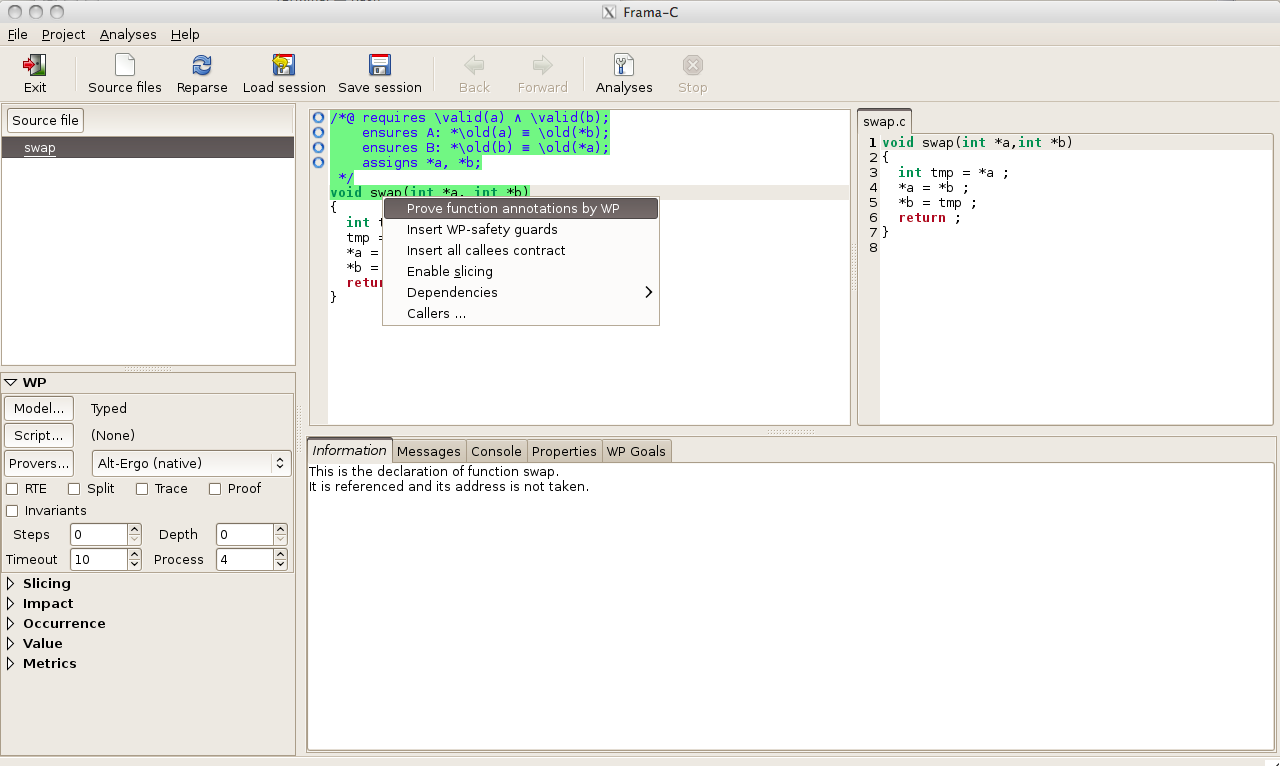
\includegraphics[width=\textwidth]{wp-gui-main.png}
\end{center}
\caption{\textsf{WP} in the Frama-C GUI}
\label{wp-gui-panel}
\end{figure}

\begin{figure}[p]
\begin{center}
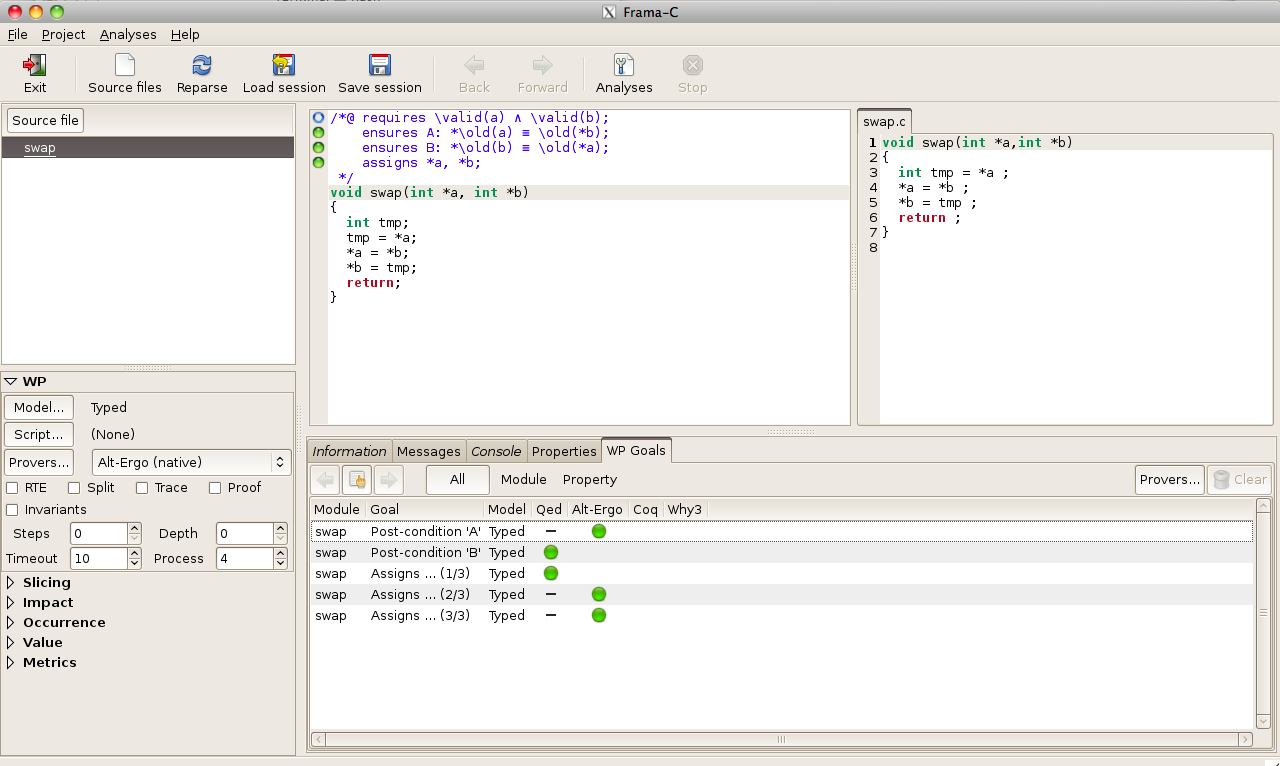
\includegraphics[width=\textwidth]{wp-gui-run.png}
\end{center}
\caption{\textsf{WP} run from the GUI}
\label{wp-gui-run}
\end{figure}

As we can see in figure~\ref{wp-gui-panel}, the memory model, the
decision procedure, and some \textsf{WP} options can be tuned from the
\textsf{WP} side panel. Other options of the \textsf{WP} plug-in are still
modifiable from the \texttt{Properties} button in the main GUI toolbar.

To prove a property, just select it in the internal source view and
choose \textsf{WP} from the contextual menu. The \texttt{Console}
window outputs some information about the
computation. Figure~\ref{wp-gui-run} displays an example of such a
session.

If everything succeeds, a green bullet should appear on the left of
the property. The computation can also be run for a bundle of
properties if the contextual menu is open from a function or behavior
selection.

The options from the \textsf{WP} side panel correspond to some options
of the plug-in command-line. Please refer to section~\ref{wp-cmdline}
for more details. In the graphical user interface, there are also
specific panels that display more details related to the \textsf{WP} plug-in,
that we shortly describe below.

\paragraph{Source Panel.} On the center of the \textsf{Frama-C} window, the status
of each code annotation is reported in the left margin. The meaning of
icons is the same for all plug-ins in \textsf{Frama-C} and more precisely described
in the general user's manual of the platform. The status emitted by the \textsf{WP} plug-in are:
\begin{center}
  \begin{tabular}{cl}
    \multicolumn{2}{l}{\bf Icons for properties:} \\
    \hline
    \loadicon{feedback/never_tried.png} & No proof attempted. \\
    \loadicon{feedback/unknown.png} & The property has not been validated. \\
    \loadicon{feedback/valid_under_hyp.png} & The property is \emph{valid} but has dependencies. \\
    \loadicon{feedback/surely_valid.png} & The property and \emph{all} its dependencies are \emph{valid}. \\
    \hline
  \end{tabular}
\end{center}

\paragraph{\textsf{WP} Goals Panel.}
This panel is dedicated to the \textsf{WP} plug-in. It shows the
generated proof obligations and their status for each prover.
By clicking on a prover
column, you can also submit a proof obligation to a prover by
hand. Right-click provides more options depending on the prover.

\paragraph{Interactive Proof Editor.}
From the Goals Panel view, you can double-click on a row and open the \emph{interactive proof editor} panel as described in section~\ref{wp-proof-editor}.

\paragraph{Properties Panel.} This panel summarizes the consolidated
status of properties, from various plug-ins. This panel is not
automatically refreshed. You should press the \texttt{Refresh} button
to update it. This panel is described in more details in the general
\textsf{Frama-C} platform user's manual.

\clearpage
%-----------------------------------------------------------------------------
\section{Interactive Proof Editor}
\label{wp-proof-editor}
%-----------------------------------------------------------------------------

This panel focus on one goal generated by \textsf{WP}, and allow the user to visualize the logical sequent to be proved, and to interactively decompose a complex proof into smaller pieces by applying \emph{tactics}.

\begin{figure}[htbp]
\begin{center}
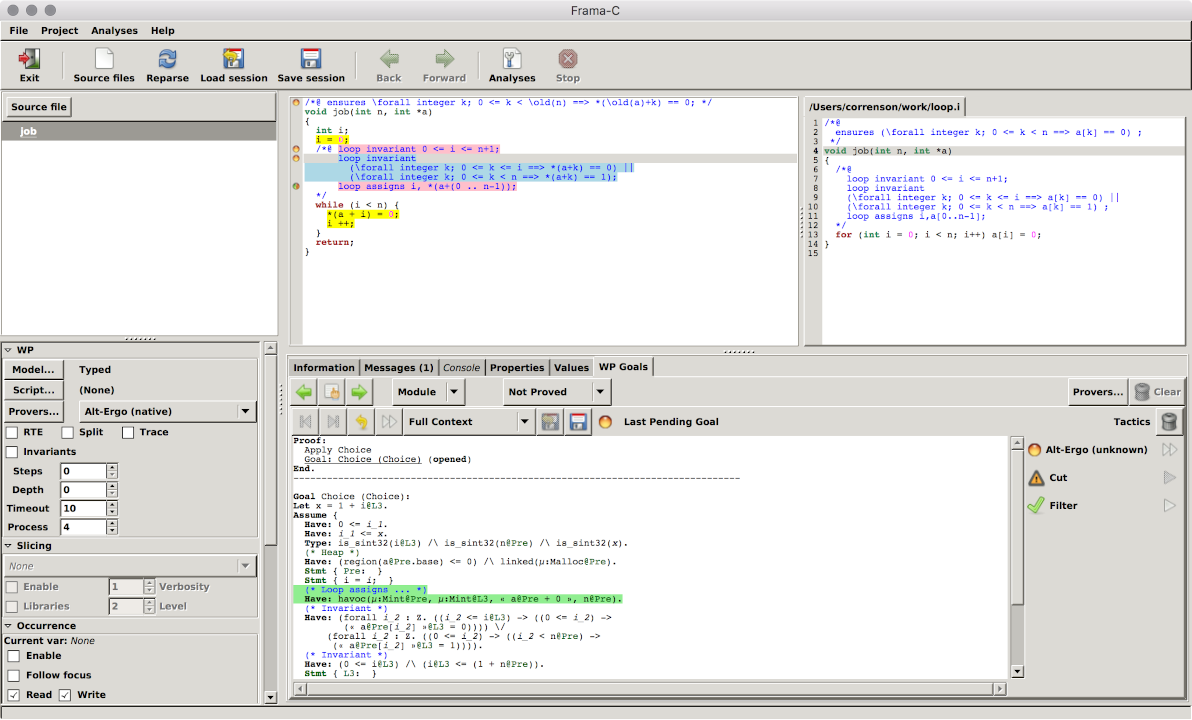
\includegraphics[width=\textwidth]{wp-tip-run.png}
\end{center}
\caption{Interactive Proof Editing}
\label{wp-tip-run}
\end{figure}

The general structure of the panel is illustrated figure~\ref{wp-tip-run}. The central text area prints the logical sequent to proved. In consists of a formula to \verb+Prove+ under the hypotheses listed in the \verb+Assume+ section. Each hypothesis can consists of :
\begin{quote}
\begin{tabular}{ll}
\verb+Type:+& formula expressing a typing constraint;\\
\verb+Init:+& formula characterizing global variable initialisation;\\
\verb+Have:+& formula from an assertion or an instruction in the code;\\
\verb+When:+& condition from a simplification performed by \textsf{Qed};\\
\verb+If:+& structured hypothesis from a conditional statement;\\
\verb+Either:+& structured disjunction from a switch statement;\\
\verb+Stmt:+& labels and C-like instructions representing memory updates in executions.\\
\end{tabular}
\end{quote}

\subsection{Display Modes}

There are several modes to display the current goal:
\begin{quote}
\begin{tabular}{ll}
\verb+Autofocus:+ & filter out clauses not mentioning \emph{focused} terms (see below);\\
\verb+Full Context:+ & disable autofocus mode --- all clauses are visible; \\
\verb+Unmangled Memory:+ & autofocus mode with low-level details of memory model; \\
\verb+Raw Obligation:+ & no autofocus and low-level details of memory model.
\end{tabular}
\end{quote}

\paragraph{Remark:} the fold/unfold operations only affect the goal display. It does not \emph{transform} the goal to be proven.

The autofocus mode is based on a ring of \emph{focused terms}. Clicking a term of a clause automatically focus this term. Shift-clicking a term adds the term to the focus ring. When autofocus mode is active, only the clauses that contains a \emph{focused} term are displayed. Hidden clauses are mentioned by an ellipsis \texttt{[...]}.

Low-level details of the memory model are normally hidden, and represented by C-like instructions such as:

\begin{ccode}
   Stmt { Label A: a.f[0] = y@Pre; }
\end{ccode}

This reads as follows: a program point is defined by the label \texttt{A}. At this point, the left-value \texttt{a.f[0]} receives the value that variable \texttt{y} holds at label \texttt{Pre}. More generally, \texttt{lv@L} means the value of l-value \texttt{lv} at label \texttt{L:}, and for more complex expression, \texttt{« e »@L} means the expression \texttt{e} evaluated at label \texttt{L}. Redundant labels are removed when possible. This is a short-hand for \textsf{ACSL} notation \lstinline{\at(e,L)} but is generally more readable.

Sometimes, some memory operations can not be rendered as C instructions, typically after transforming a goal so far. In such situations, the memory model encoding might appear with terms like \texttt{µ:Mint@L}.

With memory model unmangled, the encoding in logic formulae is revealed and no label are displayed.

\subsection{Tactics}

The right panel display a palette of tactics to be applied on the current goal. Tooltips are provided to help the user understanding how to configure and run tactics.

Only applicable tactics are displayed, with respect to current term or clause selected. Many tactics can be configured by the user to tune their effect. Click on the tactic button to toggle its control panel. Once a tactic is correctly configured, it can be applied by clicking its « Play » button.

\subsection{Term Composer}

Some tactic require one or several terms to be selected.
In such case, the normal view display the selected term.
It can be edited by buttons in the view, like a \texttt{RPN} calculator. More buttons appear with respect to already selected terms. Numerical constants can be composed, and combined with selected terms.

Typically, the composer displays a stack of values, like for instance:
\begin{ccode}
  A: 45
  B: a[0]@Pre (int)
\end{ccode}

In such a case, the user can select the value \texttt{45} with the \texttt{Select A} button, or add the two numbers with the \texttt{Add A+B} button.

Sometimes, like for the Instance tactic, a \emph{range} of numerical values can be selected. In such a case, when two numbers are selected, a special button \texttt{Select A..B} appears.

The list of all available composer buttons is displayed by the \texttt{Help} button.

A composer worth to be mentioned is \texttt{Destruct}, typically available on complex expressions. It allows to decompose a value into its sub-components. For instance, destructuring the value \texttt{B} above will reveal the address \texttt{« a+0 »@Pre} and memory \texttt{µ:Mint@Pre}.

\subsection{Proof Script}

The top toolbar upon the goal display show the current status of the goal and the number of pending goals. The media buttons allow to navigate in the proof tree.
\begin{quote}
\begin{tabular}{ll}
\verb+Next/Prev:+ & navigate among the list of pending (non proved) sub-goals; \\
\verb+Forward:+ & goes to the next pending sub-goal; \\
\verb+Backward:+ & cancel the current tactic and prover results; \\
\verb+Clear:+ & restart all the interactive proof from the initial goal.
\end{tabular}
\end{quote}

A sketch of current proof is displayed on top of the goal ; each step is clickable to navigate into the proof. Only the path leading to the current node is unfolded.

When all pending sub-goals have been proved, the initial goal is marked proved by \textsf{Tactical} in the goal list panel. It is time to save the script. A button is also available to replay the saved script, if any. Saving and replay are also accessible from the list of goals, in the popup menu of the \texttt{Script} prover column.

\subsection{Replaying Scripts}

Editing scripts interactively allows the user to finish the proofs. Once proofs are saved, he must be able to replay them from the command line. To ease the process, the following options are available to the user:
\begin{quote}
\begin{tabular}{ll}
\verb+-wp-session <dir>+ & to setup a directory where scripts are saved in; \\
\verb+-wp-prover tip+ & for incrementally building and updating the session scripts;\\
\verb+-wp-prover script+ & for replaying saved scripts only, as they are;\\
\end{tabular}
\end{quote}

The \verb+script+ prover only runs the proof scripts edited by the user from the TIP, including the scripts being complete or known to being stuck at some sub-goal. The other proof obligations are transmitted to other provers, if some are provided.

This mode is well suited for replaying a proof bench, by using a combination of provers such as \verb+-wp-prover script,Alt-Ergo+. Moreover, the \verb+script+ prover never modifies the proof session and the proof scripts.

The \verb+tip+ prover is similar, except that it never runs sub-goals that are known to be stuck but updates the proof scripts on success or when an automated proof fails. Using the \verb+tip+ prover is less time consuming and eventually prepares new scripts for failed proofs to be edited later under the TIP.

Notice that, as soon as you have setup a wp-session directory, you benefit from cache facilities to speedup your proofs. Consult Section~\ref{wp-cache} for details.

\clearpage
A typical proof session consists then in the following stages:

a. Collecting the automated proofs and preparing for the TIP.
\begin{logs}
  frama-c [...] -wp-prover tip,Alt-Ergo
\end{logs}

This runs all existing scripts (none at the very beginning) in success-mode only, and try Alt-Ergo on the others. Failed proofs lead to new empty scripts created.

b. Running the TIP.
\begin{logs}
  frama-c-gui [...] -wp-prover tip
\end{logs}

This mode only runs existing scripts (typically prepared in the previous phase) in success-mode only, which is quite fast. Finally, the GUI is opened and the user can enter the TIP and edit the proofs.

Most goals are reported not to be proved, because automated proof is deactivated since no other prover than \verb+tip+ is specified. However, by filtering only those proof scripts that requires completion, only the relevant goals appear. The user has to save its edited proof scripts to re-run them later.

Any number of phase a. and b. can be executed and interleaved. This incrementally builds the set of proof scripts that are required to complement the automated proofs.

c. Consolidating the Bench.
\begin{logs}
  frama-c [...] -wp-prover script,Alt-Ergo
\end{logs}

This mode replays the automated proofs and the interactive ones, re-running Alt-Ergo on every \textsf{WP} goals and every proof tactic sub-goals. The user scripts are never modified — this is a replay mode only.

\subsection{Tracking Scripts}

When working on large verification use-cases, it is common that some proof scripts
become useless because the associated proof obligation does not exist anymore.

WP can track the scripts that are used during verification. For this, one has to
initialize a tracking directory. This is done using the option
\verb+-wp-prepare-scripts+. This command creates a \verb+.marks+ directory in the
proof session scripts directory (that can be configured using \verb+-wp-session+),
if such a directory already exists it is removed and created again.

Then, each time WP uses a proof script, it is marked as used in the \verb+.marks+
directory. In particular, it is then possible to run WP
several times to verify different parts of the code, yet marking the scripts for
all those different parts.

Once one is certain that the entire verification of the use case has been replayed
for marking, the option \verb+-wp-finalize-scripts+ can be used to remove all
orphan scripts and the marking directory. The option \verb+-wp-dry-finalize-scripts+
can be used to log the remove actions instead of actually doing them.

\subsection{Strategies (DEPRECATED)}

\paragraph[Warning:] Strategies described below are \emph{deprecated} since Frama-C 27.0 (Cobalt).
Please use ``Proof Strategies'' instead (Section~\ref{wp-proof-strategies}).

Strategies are heuristics that generate a prioritized bunch of tactics to be tried on the current goal.
Few built-in strategies are provided by the \textsf{WP} plug-in ; however, the user can extends the proof editor with
custom ones, as explained in section~\ref{wp-custom-tactics} below.

To run strategies, the interactive proof editor provide a single button \texttt{Strategies} in the tactic panel.
Configure the heuristics you want to include in your try, then click the button. The generated with highest priority is immediately applied. The proof summary now display \texttt{backtrack} buttons revealing proof nodes where alternative tactics are available. You can use those backtracking button to cycle over the generated tactics.

Of course, strategies are meant to be used multiple times, in sequence. Recall that strategies apply highest priority tactic first, on the current goal. When using strategies several times, you shall see several \texttt{backtrack}ing buttons in your proof script. You backtrack from any point at any time.

You shall also alternate strategies \emph{and} manually triggered tactics. Though, strategies are only used to
\emph{infer} or \emph{suggest} interesting tactics to the user. Once your are finished with your proved, only the tactics are saved in the script, not the strategies used to find them. Hence, replaying a script generated with strategies would not involve backtracking any more. The script will directly replay your chosen alternatives.

It is also possible to call strategies from the command line, with option \texttt{-wp-auto}. The strategies are tried up to some depth, and while a limited number of pending goals
remains unproved by \textsf{Qed} or the selected provers. More precisely:
\begin{description}
\item[\tt -wp-auto s,...] applies strategies \texttt{s,...} recursively to unproved goals.
\item[\tt -wp-auto-depth <$n$>] limit recursive application of strategies to depth $n$ (default is 5).
\item[\tt -wp-auto-width <$n$>] limit application of strategies when there is less than $n$ pending goals (default is 10).
\item[\tt -wp-auto-backtrack <$n$>] when the first tried strategies do not close a branch, allows for backtracking
  on $n$ alternative strategies. Backtracking is performed on goals which are closed to the root proof obligation, hence
  performing a kind of width-first search strategy, which tends to be more efficient in practice.
  Backtracking is deactivated by default ($n=0$) and only used when \verb+-wp-auto+ is set.
\end{description}

The name of registered strategies is printed on console by using \texttt{-wp-auto '?'}. Custom strategies can be loaded by plug-ins, see below.

\newcommand{\TACTIC}[2]{#1\quad\quad\triangleright\quad\quad#2}

\subsection{General Tactics}

\paragraph{Absurd} Contradict the Goal or an Hypothesis\\
The user can prove the goal by contradiction:

$$ \TACTIC{\Delta\models\,G}{\Delta,\neg G\models\,\mathtt{false}} $$

Or the user can select a hypothesis $H$, and change the goal to $\neg H$:

$$ \TACTIC{\Delta,H\models\,G}{\Delta\models\,\neg H} $$

\paragraph{Clear} Remove Hypothesis\\
The user can select a hypothesis $H$, and remove it from the context:

$$ \TACTIC{\Delta,H\models\,G}{\Delta\models\,G} $$

\paragraph{Choice} Select a Goal Alternative\\
When the goal is a disjunction, the user select one alternative and discard the others:
$$ \TACTIC{\Delta\models\,\Gamma,G}{\Delta\models\,G} $$

\paragraph{Compound} Decompose compound equalities\\
When the user select an equality between two records, it is decomposed field by field.

$$ \TACTIC{ a = b }{ \bigwedge a.f_i = b.f_i } $$

\paragraph{Contrapose} Swap and Negate Hypothesis with Conclusion\\
The user select a hypothesis (typically, a negation) and swap it with the goal.
$$ \TACTIC{\Delta,H\models\,G}{\Delta,\neg G\models\,\neg H} $$

\paragraph{Cut} Use Intermediate Hypothesis
The user introduce a new clause $C$ with the composer to prove the goal. There two variants of the tactic, made available by a menu in the tactic panel.

The \textsf{Modus-Ponens} variant where the clause $C$ is used as an intermediate proof step:

$$\TACTIC{\Delta\models\,G}{%
\begin{array}[t]{ll}
\Delta &\models C \\
\Delta,C &\models G
\end{array}} $$

And the \textsf{Case Analysis} variant where the clause $C$ is used with a split:
$$\TACTIC{\Delta\models\,G}{%
\begin{array}[t]{ll}
\Delta,\phantom{\neg}C \models G \\
\Delta,\neg C \models G
\end{array}} $$

\paragraph{Definition} Unfold predicate and logic function definition\\
The user simply select a term $f(e_1,\ldots,e_n)$ or a predicate $P(e_1,\ldots,e_n)$ which is replaced by its definition, when available.

\paragraph{Filter} Dependent Erasure of Hypotheses \\
The tactic is always applicable. It removes hypotheses from the goal on a
variable used basis. When variables are compounds (record and arrays) a finer
heuristic is used to detect which parts of the variable is relevant. A
transitive closure of dependencies is also used. However, it is always
possible that too many hypotheses are removed.

The tactic also have a variant where only hypotheses \emph{not relevant} to the
goal are retained. This is useful to find absurd hypotheses that are completely
disjoint from the goal.

\paragraph{Instance} Instantiate properties\\
The user selects a hypothesis with one or several $\forall$ quantifiers, or an $\exists$ quantified goal. Then, with the composer, the use choose to instantiate one or several of the quantified parameters. In case of $\forall$ quantifier over integer, a range of values can be instantiated instead.

When instantiating hypothesis with an expression $e$:
$$\TACTIC{\Delta,\,\forall x\, P(x)\models G}{\Delta,P(e)\models G}$$

When instantiating with a range of values $n\ldots m$:
$$\TACTIC{\Delta,\,\forall x\, P(x)\models G}{\Delta,P(n)\ldots P(m)\models G}$$

When instantiating a goal with an expression $e$:
$$\TACTIC{\Delta\models \exists x\,G(x)}{\Delta\models G(e)}$$

\paragraph{Intuition} Decompose with Conjunctive/Disjunctive Normal Form\\
The user can select a hypothesis or a goal with nested conjunctions and disjunctions. The tactics then computes the conjunctive or disjunctive normal form of the selection and split the goal accordingly.

\paragraph{Lemma} Search \& Instantiate Lemma\\
The user start by selecting a term in the goal. Then, the search button in the tactic panel will display a list of lemma related to the term. Then, he can instantiate the parameters of the lemma, like with the Instance tactic.

\paragraph{Rewrite} Replace Terms\\
This tactic uses an equality in a hypothesis to replace each occurrence of term by another one.
The tactic exists with two variants: the left-variant which rewrites $a$ into $b$ from equality $a=b$,
and the right-variant which rewrites $b$ into $a$ from equality $a=b$.
The original equality hypothesis is removed from the goal.

$$\TACTIC{\Delta,a=b\models\,G}{\Delta[a\leftarrow b]\models\,G[a\leftarrow b]}$$

\paragraph{Split} Decompose Logical Connectives and Conditionals\\
This is the most versatile available tactic. It decompose merely any logical operator following the sequent calculus rules. Typically:

\[
\begin{array}{c@{\quad\quad}c@{\quad\quad}c}
  \Delta,(H_1\vee H_2)\models G & \triangleright &
     \Delta,H_1 \models G \\
  && \Delta,H_2 \models G \\
  \Delta\models(G_1\wedge G_2) & \triangleright &
     \Delta\models G_1 \\
  && \Delta\models G_2 \\
  \Delta,H?P:Q\models G & \triangleright &
     \Delta,\phantom{\neg}H,P\models G \\
  && \Delta,\neg H,Q\models G \\
  \ldots
\end{array}
\]

When the user selects a arbitrary boolean expression $e$, the tactic is similar to the Cut one:
\[\TACTIC{\Delta\models\,G}{%
\begin{array}[t]{l}
\Delta,\phantom{\neg}e\models G \\
\Delta,\neg e\models G
\end{array}} \]

Finally, when the user select a arithmetic comparison over $a$ and $b$,
the tactics makes a split over $a=b$, $a<b$ and $a>b$:
\[\TACTIC{\Delta\models\,G}{%
\begin{array}[t]{ll}
\Delta,a<b&\models G \\
\Delta,a=b&\models G \\
\Delta,a>b&\models G
\end{array}} \]

\subsection{Integers \& Bit-wised Tactics}

\paragraph{BitRange} Range of logical bitwise operators \\
This tactical applies the two following lemmas to the current goal.
The first lemma is on logical-or, and only applies to positive integers:
\[
\begin{array}{c}
  \bigwedge_i 0 \leq x_i < 2^p
  \\\hline
  0 \leq \mathtt{lor}(x_1,\ldots,x_n) \leq 2^p
\end{array}
\]

The second lemma is on logical-and, and applies to at-least one positive integer:
\[
\begin{array}{c}
  \bigvee_i 0 \leq x_i \quad\wedge\quad \bigwedge_i x_i \leq 2^p
  \\\hline
  0 \leq \mathtt{land}(x_1,\ldots,x_n) \leq 2^p
\end{array}
\]

The tactical rewrites range goals on logical and/or into the corresponding range over its parameters, by finding a suitable $2^p$
to apply the theorems. Such a strategy is \emph{not} complete in general.
Typically, $\mathtt{land}(x,y) < 38$ is true whenever both $x$ and $y$ are in range $0\ldots 31$, but this is also true
in other cases.

\paragraph{Bit-Test Range} Tighten bounds with respect to bits \\
The \lstinline{bit_test(a,b)} function is predefined in \textsf{WP} and is equivalent
to the \textsf{ACSL} expression \lstinline{(a & (1 << k)) != 0}. The
\textsf{Qed} engine has many simplification rules that applies to
such patterns.

The user selects an expression $\mathtt{bit\_test}(n,k)$ with $k$
a \emph{constant} integer value greater or equal to 0 and lower than
128. The tactic uses this test to thighten the bounds of $n$.

$$\TACTIC{\Delta\models\,G}{%
\begin{array}[t]{ll}
\Delta,T &\models G \\
\Delta,F &\models G
\end{array}} $$

with
$$\begin{array}[t]{rlcll}
  T \equiv & \mathtt{bit\_test}(n,k) & \wedge & (0 \leq n & \Rightarrow 2^{k} \leq n) \\
  F \equiv & \neg \mathtt{bit\_test}(n,k) & \wedge & (0 \leq n < 2^{k+1} & \Rightarrow n < 2^{k})
  \end{array}
$$

\paragraph{Bitwise} Decompose equalities over $N$-bits\\
The use selects an integer equality and a number of bits.
Providing the two members of the equality are in range $0..2^N-1$,
the equality is decomposed into $N$ bit-tests equalities:
\[\TACTIC{\Delta\models G}{%
\begin{array}[t]{rcl}
\Delta\phantom{)} &\models & 0 \leq a,b < 2^N \\
\sigma(\Delta) & \models & \sigma(G)
\end{array}
}\]
where $\sigma$ is the following subsitution:
\[ \sigma \equiv
\left[ a=b \quad \leftarrow
\bigwedge_{k\in 0..N-1} \mathtt{bit\_test}(a,k) = \mathtt{bit\_test}(b,k)
\right]
\]

\paragraph{Congruence} Simplify Divisions and Products \\
This tactic rewrites integer comparisons involving products and divisions.
The tactic applies one of the following theorems to the current goal.
In the following lemmas, $k$, $k'$, and $n$ are integer constants, $a$ and $b$ any integer terms.
The notation $k|n$ stands for $k$ divides $n$.
The lemmas are extended to non-strict inequalities and non-positive constants in a natural way.
\[
\begin{array}{crcl}
0<k, & a < n/k &\Longrightarrow& k.a < n \\
k|n, & a = n/k &\Longleftrightarrow& k.a = n \\
\neg(k|n), & k.a = n & \Longrightarrow & \mathtt{false} \\
0<k, & a < k.(b+1) &\Longrightarrow& a/k < b \\
0<k, 0<k', & k'.a < k.b &\Longrightarrow& a/k < b/k' \\
n|k, n|k', & (k/n).a = (k'/n).b &\Longleftrightarrow& k.a = k'.b
\end{array}
\]

\paragraph{Induction} Start a proof by integer induction \\
The user select any integer expression $e$ in the proof and a base value $b$ (which defaults to
0). The tactic generates a proof by induction on $e$, that is, the base case
$e = b$ and then the cases $e < b$ and $b < e$. Formally, the initial goal
$\Delta_0\models\,G_0$ is first generalized into $\Delta,P(e)\models\,Q(e)$. The tactic
then proceed by (strong) induction over $n$ for
$G(n) \equiv P(n)\Longrightarrow\,Q(n)$:

\[\TACTIC{\Delta\models\,G(n)}{%
\begin{array}[t]{lll}
\Delta,\; \quad n = b & \models G(n) \\
\Delta,\; \forall i,\, b \leq i < n \Longrightarrow G(i) \; & \models G(n) \\
\Delta,\; \forall i,\, n < i \leq b \Longrightarrow G(i) \; & \models G(n)
\end{array}} \]

\paragraph{Mod-Mask} Rewrite bitmask into/from modulo \\
This tactic is used to rewrite a bitmask into a modulo (or a modulo into a
bitmask) when possible. The user selects an expression $e$ of the form
$b \% m$ (resp. $b \& m$ - $\texttt{land b m}$) than can be rewritten into
$b \& (m+1)$ (resp. $b \% (m - 1)$), if $0 \leq b$ and $m$ is a positive power
of 2 (resp. $m + 1$ is a positive power of 2). When selecting an expression
$x \& y$, both directions $x \% (y - 1)$ and $y \% (x - 1)$ can be considered.

Since establishing that $m$ is a positive power of 2 can be hard, the tactic has
several behaviors. If \textsf{Qed} can prove immediately that an operand $m$ (or
$m+1$ for bitmaks) is a positive power of 2, the tactic only generates the guard
$0 \leq b$ and the rewritten goal. If it is not the case, the tactic appears
with the name ``Mod-Mask (hard)'' in the GUI. In this situation, the guard
consists of two conditions: $0 \leq b$ and $m$ (or $m+1$) is a positive power of
2. This guard involves an existential quantification, so it can be hard to
prove. When the selected term is a bitmask, the tactic cannot decide itself the
direction of the modulo, thus a checkbox is added in the configuration of the
tactic to select the direction of rewriting.

\paragraph{Overflow} Integer Conversions \\
This tactic split machine integer conversions into three cases: value in integer
range, lower than range and upper than range. The tactic applies on expression
with pattern $\mathtt{to\_iota(e)}$ where \texttt{iota} is a machine-integer type
name, \emph{eg.} \texttt{to\_uint32}.

\[\TACTIC{\Delta\models G}{%
\begin{array}[t]{rcl}
\sigma_{id}(\Delta) & \models & low \leq e \leq up \Rightarrow \sigma_{id}(G) \\
\sigma_{+}(\Delta) & \models & low < e \Rightarrow \sigma_{+}(G) \\
\sigma_{-}(\Delta) & \models & e < up \Rightarrow \sigma_{-}(G)
\end{array}
}\]
where
\begin{itemize}
  \item $[low..up]$ is the range of the \texttt{iota} integer domain,
  \item $\sigma_{id} = [ \mathtt{to\_iota}(e) \mapsto e ]$,
  \item $\sigma_{+}  = [ \mathtt{to\_iota}(e) \mapsto \mathtt{overflow}(e) ]$,
  \item $\sigma_{-}  = [ \mathtt{to\_iota}(e) \mapsto \mathtt{overflow}(e) ]$.
\end{itemize}

\paragraph{Range} Enumerate a range of values for an integer term\\
The user select any integer expression $e$ in the proof, and a range of numerical values $a\ldots b$. The proof goes by case for each $e=a\ldots e=b$, plus the side cases $e<a$ and $e>b$:
$$\TACTIC{\Delta\models\,G}{%
\begin{array}[t]{ll}
\Delta,e<a &\models G \\
\Delta,e=a &\models G \\
&\vdots \\
\Delta,e=b &\models G \\
\Delta,e>b &\models G
\end{array}} $$

\paragraph{Shift} Transform logical shifts into arithmetics\\
For positive integers, logical shifts such as \lstinline{a << k}
and \lstinline{a >> k} where \lstinline$k$ is a constant can be interpreted into a multiplication or a division by $2^k$.

When selecting a logical-shift, the tactic performs:
\[\TACTIC{\Delta\models G}{%
\begin{array}[t]{rcl}
\Delta\phantom{)} &\models& 0 \leq a \\
\sigma(\Delta) &\models& \sigma(G)
\end{array}
}\]
where:
\begin{tabular}[t]{ll}
$\sigma = [ \mathtt{lsl}(a,k) \leftarrow a * 2^k ]$ &
for left-shift, \\
$\sigma = [ \mathtt{lsr}(a,k) \leftarrow a / 2^k ]$ &
for right-shifts.
\end{tabular}

\subsection{Domain Specific Tactics}

\paragraph{Array} Decompose array access-update patterns\\
The use select an expression $e\equiv a[k_1\mapsto v][k_2]$. Then:

\[
\TACTIC{\Delta\models\,G}{%
\begin{array}[t]{ll}
\Delta,\,k_1=k_2,\,e = v &\models G \\
\Delta,\,k_1\neq k_2,\,e = a[k_2] &\models G
\end{array}
}\]

\paragraph{Havoc} Go Through Assigns \\
This is a variant of the \texttt{Lemma} tactic dedicated to \texttt{Havoc} predicate generate by complex assigns clause. The user select an address, and if the address is not assigned by the \texttt{Havoc} clause, the memory at this address is unchanged.

\paragraph{Separated} Expand Separation Cases\\
This tactic decompose a \texttt{separated}$(a,n,b,m)$ predicate into its four base cases: $a$ and $b$ have different bases, $a+n \leq b$, $b+m \leq a$, and $a[0..n-1]$ and $b[0..m-1]$ overlaps. The regions are separated in the first three cases, and not separated in the overlapping case. This is kind of normal disjunctive form of the separation clause.


\paragraph{Sequence} Unroll repeat-sequence operator\\
In this section, let us use $A^n$ for the ACSL notation \lstinline{A *^ n},
the repeat list operation, and $A \oplus l$ for the list concatenation.

This tactics is used to transform $A^n$ sequences. Threes behaviors
can be selected:
unroll left that rewrites the list  $A^n$ into $A \oplus A^{n-1}$,
unroll right that rewrites the list $A^n$ into $A^{n-1} \oplus A$
and unroll sum that rewrites the list $A ^{n_1 + ... + n_k}$
into $A^{n_1} \oplus ... \oplus A^{n_k}$. For unroll left and right,
a negative value leads to an empty list. For unroll sum, one must prove that all
$nI$ are positive.

Rule for unroll left:

\[
\TACTIC{\Delta\models\,G}{%
\begin{array}[t]{lll}
  \Delta[A^n\leftarrow A \oplus A^{n-1}],& n > 0 & \models G[A^n\leftarrow A \oplus A^{n-1}]\\
  \Delta[A^n\leftarrow []],& n \leq 0 & \models G[A^n\leftarrow []]
\end{array}
}\]

Rule for unroll right:

\[
\TACTIC{\Delta\models\,G}{%
\begin{array}[t]{lll}
  \Delta[A^n\leftarrow A^{n-1} \oplus A],& n > 0 & \models G[A^n\leftarrow A^{n-1} \oplus A]\\
  \Delta[A^n\leftarrow []],& n \leq 0 & \models G[A^n\leftarrow []]
\end{array}
}\]

Rule for unroll sum:

\[
\TACTIC{\Delta\models\,G}{%
\begin{array}[t]{ll}
  \Delta & \models\bigwedge_{i=1}^{k} 0 \leq n_i\\
  &\\
  \Delta[A^{\sum_{i=1}^{k}n_i}\leftarrow \bigoplus_{i=1}^{k} A^{n_i}] &
  \models G[A^{\sum_{i=1}^{k}n_i}\leftarrow \bigoplus_{i=1}^{k} A^{n_i}]
\end{array}
}\]

\paragraph{Validity} Unfold validity and range definitions\\
The user selects a validity expression (\lstinline{valid_rd},
\lstinline{valid_rw}, \lstinline{invalid} or \lstinline{included}).
The expression is unfolded to a \textsf{Qed} term.


\subsection{Custom Tactics and Strategies}
\label{wp-custom-tactics}

The proof editor and script runner can be extended by loading additional plug-ins. These plug-ins are regular OCaml files to be loaded with the kernel \texttt{-load-module} option. They will be compiled by \textsf{Frama-C} against its API. The \textsf{WP} plug-in exports a rich API to extend the proof editor with new tactics, strategies, and even term-composer tools.

It is not possible to reproduce here the complete API ; it is better to use the automatically generated HTML documentation from \textsf{WP}'s sources. We only provide here a quick tour of this API, as a tutorial on how to implement a basic custom strategy.

The main extension points of the \textsf{WP} plug-in's API are the following ones:
\begin{center}
    \begin{tabular}{ll}
    \hline
    \texttt{Wp.Tactical.tactical} & Base-class definition of custom Tactic. \\
    \texttt{Wp.Strategy.heuristic} & Base-class definition of custom Strategy. \\
    \hline
    \texttt{Wp.Auto.$\star$} & Pre-defined tactics and strategies. \\
    \texttt{Wp.Tactical.register} & Registration point for custom Tactics. \\
    \texttt{Wp.Strategy.register} & Registration point for custom Strategies. \\
    \texttt{Wp.Tactical.add\_composer} & Registration point for custom term composer. \\
    \hline
    \end{tabular}
\end{center}

\paragraph{Warning:} It is technically possible to break the logical soundness of \textsf{WP} when using custom tactics crafted by hand. Fortunately, using only pre-defined tactics in custom strategies will be always safe, even if your heuristic generates crazily stupid alternatives to solve a goal. The point with custom \emph{tactics} is that you might transform a sequent \emph{without preserving} the equivalence with the original goal if you make some mistakes into your custom code. This is the same problem as using \textsf{ACSL} axioms instead of lemmas. So, use custom tactics carefully, and prefer custom strategies when possible.

To build a custom strategy, the typical boilerplate code is as follows:
\begin{lstlisting}[language=ocaml]
 (* file: dummy.ml *)
open Wp

class dummy : Strategy.heuristic =
object
    method id = "MyStrategy.dummy" (* required, must be unique *)
    method title = "Split Goal"    (* visible in Strategy panel *)
    method descr = "Simply split conjunctions in goal" (* idem *)
    method search push sequent = (* heuristic code *)
      let goal = snd sequent in
      match Repr.pred goal with
      | And _ ->
          let selection = Tactical.(Clause(Goal goal)) in
          push (Auto.split ~priority:2.0 selection)
      | _ -> ()
end

(* Register the strategy *)
let () = Strategy.register (new dummy)
\end{lstlisting}

Then, simply extend your command line with the following options to make your strategy available from the interactive proof editor:
\begin{logs}
> frama-c-gui -load-module dummy.ml [...]
\end{logs}

\paragraph{Note:} Loading custom strategies is only required when running the graphical user interface (\texttt{frama-c-gui}). When replaying scripts from the command line (\texttt{frama-c}), only custom tactics and custom composers actually involved in proofs are required to be loaded.

The example custom strategy above is structured as follows. First we open the module \lstinline$Wp$ to simplify
access to the API. A custom strategy must be an instance of class-type \lstinline$Strategy.heuristic$, and we use a coercion here to explicit types. Methods \lstinline$#id$, \lstinline$#title$ and \lstinline$#descr$ are required and describes the strategy, making it available from the tactic panel in the graphical user interface.

The actual heuristic code takes place in method \lstinline$#search$ which has the following type (consult the html API for details):
\begin{lstlisting}[language=ocaml]
method search :
  (Strategy.strategy -> unit) -> Conditions.sequent -> unit
\end{lstlisting}

This method takes two parameters: a strategy registration callback and the sequent to prove. Each heuristic
is supposed to register any number of strategies to be tried on the provided sequent. In turn, each strategy
is a record consisting of a priority, a tactic, a target selection for the tactic and its arguments.
It is possible to build such a record by hand, using custom or predefined tactics. However, it is much more convenient
to use the helper functions from module \lstinline$Auto$ that directly build strategies.

In the example above, we inspect the structure of the goal, and when a conjunction is detected (\lstinline$And _$),
we decide to register a split tactic, thanks to the helper function \lstinline$Auto.split$. Default priority is \lstinline$1.0$ by convention. Pre-installed strategies would only use range $[0.5\ldots2.0]$ of priorities. You can use any value you want inside or outside this range. In the example below, we assign a high priority to the split of goal conjunctions, meaning that such a split should be tried first.

\paragraph{Using Selections.} Tactics always need a \lstinline$selection$ target. Moreover, some tactics require additional parameters, also to be provided as \lstinline$selection$ values. Typically, consider the \lstinline$Auto.range$ tactic:

\begin{lstlisting}[language=ocaml]
val Auto.range :
  ?priority:float -> selection -> vmin:int -> vmax:int -> strategy
\end{lstlisting}

Here the selection argument shall targets the expression to be enumerated in range \lstinline$vmin..vmax$.
Selections must refer to a term that pre-exists in the sequent. You must indicate to the \textsf{WP} proof engine
how to rebuild this term from the sequent. Hence, if the \textsf{C}-code or the \textsf{ACSL} specification change,
\textsf{WP} still has a chance to rebuild the same selection from the updated sequent.

Selections are easy to build. There are five basic forms, as described below:
\begin{lstlisting}[language=ocaml]
   type Tactical.selection =
     | Empty
       (** no selection *)
     | Clause of clause
       (** selects a full hypothesis or the full goal *)
     | Inside of clause * Lang.F.term
       (** selects a sub-term of a hypothesis or goal *)
     | Compose of compose
       (** a calculus from several sub-selections *)
   and Tactical.clause =
     | Goal of Lang.F.pred
     | Step of Conditions.step
\end{lstlisting}

It is also possible to build selections from sequent by explicit lookup:
\begin{lstlisting}[language=ocaml]
   val Strategy.select_e :
     Conditions.sequent -> Lang.F.term -> Tactical.selection
   val Strategy.select_p :
     Conditions.sequent -> Lang.F.pred -> Tactical.selection
\end{lstlisting}

Composition allows you to build new terms from existing ones, like when using the term composer from the graphical user interface. You access composers by their name, like in the term composer. The API for building new terms is as follows:
\begin{lstlisting}[language=ocaml]
   val Tactical.int :
     int -> Tactical.selection
   val Tactical.cint :
     Integer.t -> Tactical.selection
   val Tactical.range :
     int -> int -> Tactical.selection
   val Tactical.compose :
     string -> Tactical.selection list -> Tactical.selection
\end{lstlisting}

For instance, provided you have two selected terms \lstinline$a$ and \lstinline$b$, you can build their sum using
\lstinline$compose "wp:add" [a;b]$. The name of composers can be obtained from the graphical user interface.

\paragraph{Exploring Sequents.}
The clauses refer to parts of the provided sequent. Typically, a sequent consists of a
sequence of hypothesis, and a goal to prove. Each hypothesis is represented by a \lstinline$step$, consisting either of single hypothesis or a more structured condition
(branch, cases, \textit{etc}.):

\begin{lstlisting}[language=ocaml]
   type Conditions.sequent = sequence * Lang.F.pred
   and  sequence = .... step list ... (* private type *)
   and  step = { condition : condition ; ... }
   and  condition =
     | Have of Lang.F.pred (** Hypothesis *)
     | Init of Lang.F.pred (** C-initializer initialization clause *)
     | Type of Lang.F.pred (** C/ACSL type constraints *)
     | Core of Lang.F.pred (** Common hypothesis factorization from WP *)
     | When of Lang.F.pred (** Hypothesis (tactical or simplification) *)
     | Branch of Lang.F.pred * sequence * sequence (** If-Then-Else *)
     | Either of sequence list (** Disjunction of Cases *)
   val iter : (step -> unit) -> sequence -> unit
\end{lstlisting}

When you walk through a sequence of hypothesis, you shall reuse the provided steps to build clauses and selections.

\paragraph{Exploring Formulae}.
The constituent of hypothesis and goals are logical terms and predicates. You shall use
module \lstinline$Repr.term$ and \lstinline$Repr.pred$ to access the internal representation
of formulae. There are many constructors for terms and predicates, simply browse the html documentation to have an overview. Many properties about terms and predicates are directly obtained from the \lstinline$Lang.F$ module. The API is quite rich, so use the html documentation to get details.

\clearpage
%-----------------------------------------------------------------------------
\section{Command Line Options}
\label{wp-cmdline}
%-----------------------------------------------------------------------------

The best way to know which options are available is to use:
\begin{shell}
# frama-c -wp-help
\end{shell}

The \textsf{WP} plug-in generally operates in three steps:
\begin{enumerate}
\item Annotations are selected to produce a control-flow graph of
  elementary statements annotated with hypotheses and goals.
\item Weakest preconditions are computed for all selected goals in the
  control-flow graph. Proof obligations are emitted and saved on disk.
\item Decision procedures (provers) are run to discharge proof obligations.
\end{enumerate}

The \textsf{WP} options allow to refine each step of this process. It
is very convenient to use them together with the standard \texttt{-then}
option of \textsf{Frama-C}, in order to operate successive passes on the project.
See section~\ref{wp-persistent} for details.

\subsection{Goal Selection}

This group of options refines the selection of annotations for which
proof obligations are generated. By default, all annotations are
selected. A property which is already proved -- by \textsf{WP} or by
any other plug-in -- does not lead to any proof-obligation generation,
unless the property is individually selected from the graphical user
interface of the programmatic API.

\begin{description}
\item [\tt -wp] generates proof obligations for all (selected) properties.
\item [\tt -wp-fct <f$_1$,...,f$_n$>] selects annotations of functions
  \texttt{f$_1$},...,\texttt{f$_n$} (defaults to all functions).
\item [\tt -wp-skip-fct <f$_1$,...,f$_n$>] ignores
  functions \texttt{f$_1$},...,\texttt{f$_n$} (defaults to none).
\item [\tt -wp-bhv <b$_1$,...,b$_n$>] selects annotations for behaviors
  \texttt{b$_1$},...\texttt{b$_n$} (defaults to all behaviors) of the
  selected functions (the name \texttt{default!} can be used to select
  the default anonymous behavior).
\item [\tt -wp-prop <p$_1$,...,p$_n$>] selects properties having
  \texttt{p$_1$} or ...\texttt{p$_n$} as tagname (defaults to all
  properties). You may also replace a tagname by a
    \texttt{@<category>} of properties.
    \\
    Recognized categories are: \texttt{@lemma}, \texttt{@requires}, \texttt{@assigns},
    \texttt{@ensures}, \texttt{@exits}, \texttt{@assert}, \texttt{@check},
    \texttt{@invariant}, \texttt{@variant}, \texttt{@breaks},
    \texttt{@continues}, \texttt{@returns}, \texttt{@terminates},\\
    \texttt{@decreases},
    \texttt{\mbox{@complete\_behaviors}}, \texttt{\mbox{@disjoint\_behaviors}}.
    \\
    Tags and categories can be prefixed with a minus sign to \emph{skip}
    the associated annotations.
    For example \texttt{-wp-prop="-@assigns"} removes all \texttt{assigns}
    and \texttt{loop assigns} properties from the selection.
    \\
    Tag names also include the name of the function or
    lemma associated with the property.
    \\
    \textbf{Remark:} properties with tag name \verb+no_wp:+ are always and automatically
    filtered out and never proved by \textsf{WP}.
\item [\tt -wp-(no)-status-all] includes in the goal selection all properties
  regardless of their current status (default is: \texttt{no}).
\item [\tt -wp-(no)-status-valid] includes in the goal selection those properties
  for which the current status is already 'valid' (default is: \texttt{no}).
\item [\tt -wp-(no)-status-invalid] includes in the goal selection those properties
  for which the current status is already 'invalid' (default is: \texttt{no}).
\item [\tt -wp-(no)-status-maybe] includes in the goal selection those properties with
  an undetermined status (default is: \texttt{yes}).
\item [\tt -wp-(no)-legacy] use the legacy WP generator, if set to \texttt{no},
  WP uses a recently developed generator (default is: \texttt{no}).
\item [\tt -wp-dump] does not prove selected properties, but dumps the control
  flow graph computed by WP, including code annotations, both DOT files and PDF
  files into the directory specified by \texttt{-wp-out}.
\end{description}

\textbf{Remark:} options \texttt{-wp-status-xxx} are not taken into account
when selecting a property by its name or from the GUI.

\subsection{Program Entry Point}

The generic \textsf{Frama-C} options dealing with program entry point
are taken into account by \textsf{WP} plug-in as follows:

\begin{description}
\item [\tt -main <f>] designates \texttt{f} to be the main entry point (defaults to \texttt{main}).
\item [\tt -lib-entry] the main entry point (as defined by option
\texttt{-main}) is analyzed regardless of its initial context (default is no).
\end{description}

These options impact the generation of proof-obligations for the
``\texttt{requires}'' contract of the main entry point. More precisely, if there
is a main entry point, \emph{and} \texttt{-lib-entry} is not set:
\begin{itemize}
\item the global variables are set to their initial values at the
  beginning of the main entry point for all its properties to be established;
\item special proof obligations are generated for the preconditions of the
  main entry point, hence to be proved with globals properly initialized.
\end{itemize}

Otherwise, initial values for globals are not taken into account and
no proof obligation is generated for preconditions of the main entry
point.

\subsection{Model Selection}
These options modify the underlying memory model that is used for
computing weakest preconditions. See chapter~\ref{wp-models} for
details. Models are identified by a combination of \emph{selectors}
which are defined below:
\begin{center}
  \begin{tabular}{cl}
    Selector & Description \\
    \hline
    \texttt{\bf Hoare} & Select Hoare memory model. \\
    \texttt{\bf Typed} & Select Typed memory model with limited casts.\\
    \texttt{cast}  & Select Typed memory model with unlimited casts (unsound). \\
    \texttt{nocast} & Select Typed memory model with \emph{no} casts. \\
    \hline
    \texttt{raw} & Disable the combination of memory models. \\
    \texttt{var} & Combination of memory models based on variable analysis. \\
    \texttt{ref} & Activate the detection of pointer variables used for reference passing style. \\
    \texttt{caveat} & Caveat memory model (see~\ref{CAVEAT}). \\
    \hline
    \texttt{int} & Use machine integers when overflows and downcasts might occurs. \\
    \texttt{nat} & Integer model without bounds (no overflow assumed). \\
    \hline
    \texttt{float} & Use floating-point operations. \\
    \texttt{real} & Use mathematical reals instead of floating point. \\
    \hline
  \end{tabular}
\end{center}

Refer to Section~\ref{wp-model-arith} for details on arithmetic models and
Chapter~\ref{wp-models} for a description of memory models.

The available \textsf{WP} command-line options related to model selection are:
\begin{description}
\item[\tt -wp-model <spec...>] specifies the models to use. The
  specification is a list of \emph{selectors}. Selectors are usually
  separated by `\verb|,|' although other separators are accepted as well:
  `\verb|+|', `\verb|_|', spaces, newlines, tabs and parentheses `\verb|(|',
  `\verb|)|'.\\ Selectors are \emph{case insensitive}. The option
  \texttt{-wp-model} can be used several times. All provided selectors
  are processed from left to right, possibly canceling previous ones.\\
  Default setting corresponds to \texttt{-wp-model "Typed+var+int+float"}.

\item[\tt -warn-(un)signed-(overflow|downcast)] those kernel options are
  used by the (default) arithmetic model \texttt{-wp-model +int} to interpret integer
  arithmetic. See section~\ref{wp-model-arith} for details.

\item[\tt -wp-literals] exports the contents of string literals
  to provers (default: \texttt{no}).
\item[\tt -wp-extern-arrays] gives an arbitrary large size to arrays
  with no dimensions. This is a model of infinite size arrays
  (default is: \texttt{no}).
\item[\tt -wp-(alias|unalias|ref|context)-vars <var,...>] these options can be used
  to finely tweak the memory model inferred by \textsf{WP}. Each variable with a given name
  can be forced to be modeled as follows:\\[1ex]
  \begin{tabular}{rl}
      \texttt{alias}: & the variable is known to have aliases and modeled by \texttt{Typed}.\\
      \texttt{noalias}: & the variable is known to have \emph{no} alias and modeled with \texttt{Hoare}.\\
      \texttt{ref}: & the variable is a constant pointer and is modeled by the \texttt{Ref}.\\
      \texttt{context}: & the variable is initially non-aliased and uses a fresh global in \texttt{Typed}.\\
  \end{tabular}
\item[\tt -wp-(no)-alias-init] Use initializers for aliasing propagation (default is: yes).
\item[\tt -wp-(no)-volatile] this option (de)activate the correct handling of
  volatile access. By default, accessing a volatile l-value returns an undefined
  value, and writing to a volatile l-value is modeled like an \textsf{ACSL} assigns clause.
  Hence, only the accessed \emph{values} are ignored.\\
  Setting \texttt{-wp-no-volatile} turns this behavior off: it is potentially \emph{unsound} and
  makes the \textsf{WP} emitting a warning on each volatile access.
\item[\tt -wp-(no)-warn-memory-model] this option (de)activate the
  warnings about memory model hypotheses
  for the generated proof obligations, as described in Section~\ref{wp-model-hypotheses}.
  For each model supporting this feature, and each concerned function,
  an \textsf{ACSL} specification is printed on output.
  Currently, only the \texttt{Caveat}, \texttt{Typed} and \texttt{Ref} memory models support
  this feature. See also experimental option below.
\item[\tt -wp-(no)-check-memory-model] this \emph{experimental} option generates
  ACSL contracts for the selected memory model hypotheses, as described
  in Section~\ref{wp-model-hypotheses} and listed by option
  \texttt{-wp-warn-memory-model}.
  Hence, the memory model hypothes are exposed to \textsf{WP} and other plugins.
  Disabled by default.
\end{description}

\subsection{Computation Strategy}
\label{subsec:computation-strategy}

These options modify the way proof obligations are generated during
weakest precondition calculus.

\begin{description}
\item[\tt -wp-(no)-rte] generates RTE guards before computing weakest
  preconditions. This option calls the \emph{rte generation} plug-in
  before generating proof obligations.
  The generated guards, when proved\footnote{It is still correct to prove these RTE
    annotations with the \textsf{WP} plug-in.}, fulfill the requirements for
  using the \textsf{WP} plug-in with the default machine-integer domain (default is: \texttt{no}).
  Using this option with \texttt{-wp-model nat} is tricky, because \texttt{rte} uses the kernel options
  to generate guards, and they might be not strong enough to meet the natural model requirements.
  In this case, a warning is emitted for potential runtime errors.
  Refer to Section~\ref{wp-model-arith} for details.
\item[\tt -wp-(no)-init-const] use initializers for global const variables
  (defaut is: \texttt{yes}).
\item[\tt -wp-(no)-split] Splits conditional statements into separated goals (default is: \texttt{no}).
\item[\tt -wp-(no)-split-switch] Splits switch statements into sepeared goals (default is: \texttt{yes}).
\item[\tt -wp-split-max <{\it n}>]
  limits the number of sub-goals generated by  \verb|-wp-split| and \verb|-wp-split-switch|
  (defaults to \verb+1000+).
\item[\tt -wp-(no)-split-conj] conjunctions in generated proof obligations are
  recursively split into sub-goals.  The generated goal names are
  suffixed by ``{\tt part<{\it n}>}'' (defaults to \texttt{no}).
\item[\tt -wp-split-cnf <{\it d}>] transforms all goals with in conjunctive normal form (CNF) at depth {\tt\it d}.
  Value \verb|-1| stands for unlimited depth. Default is 0, which means no CNF transformation.
\item[\tt -wp-(no)-callee-precond] includes preconditions of the callee
  after\footnote{Proof obligations are always generated to check preconditions.}
  a call (default is: \texttt{yes}).
\item[\tt -wp-(no)-precond-weakening] discard pre-conditions of side behaviours (sound but
  incomplete optimisation, default is: \texttt{no}).
\item[\tt -wp-unfold-assigns <{\it n}>] when proving assigns, unfold up to
  \textit{n} levels of \texttt{struct} compounds types or access via ranges.
  \texttt{struct} are unfolded field by field, ranges are unfolded cell by
  cell (via a universal quantification over the index of the cell).
  This allows for proving that assigning a complete structure is still included
  into an assignment field by field, or that assigning a range is still included
  in a union of subranges. This option is set to \texttt{0} by default, because
  it is generally not necessary and it can generates a large number of
  verifications for structures with many (nested) fields. \texttt{-1} enables
  full unfolding.
\item[\tt -wp-(no)-variant-with-terminates] prove \texttt{loop variant} under
  the termination hypothesis (thus, under a
  \texttt{terminates \textbackslash{}false}, any loop variant proof is trivial)
  (default is: \texttt{no}).
\end{description}

\subsubsection{ACSL extension \texttt{@calls}}
\label{acsl:calls}

Frama-C provides an ACSL extension \texttt{@calls} that can be written
before an indirect call to indicate which functions can be the target
of the pointer (see \cite{userman} for more information). Upon encountering
such annotation, WP will perform a case analysis with the contract of
each provided function.

For example:

\begin{lstlisting}[style=c]
/*@ ensures \result == x ; */
int f1(int x);
/*@ ensures \result == x+1 ; */
int f2(int x);

/*@ requires fp == &f1 || fp == &f2 ;
    ensures POST: \result == 4 || \result == 5; */
int caller(int (*fp)(int)){
  //@ calls f1, f2 ;
  return (*fp)(4);
}
\end{lstlisting}

These annotations split post-conditions to the dynamic call into two sub-goals: one for call to \verb+f1+ and
a second for the call to \verb+f2+. A last goal is generated at the call
site: one must prove that \verb+fp+ is either \verb+f1+ or \verb+f2+.

\subsubsection{Proof of \texttt{@terminates}}
\label{ss-sec:plugin-terminates}

In ACSL, a function can be specified to terminate when some condition \verb+P+ holds
in pre-condition.

\begin{lstlisting}[style=c]
/*@ terminates P ; */
void function(void){
  ...
}
\end{lstlisting}

If terminates verification is active (depending on \verb+-wp+ options) WP collects all function calls and loops
and generate verification conditions (VCs) to prove them, as detailed below.

\paragraph{Loop variants.} When a loop has a variant, no particular verification
is generated for termination. However, if \verb+-wp-variant-with-terminates+ is
active, the variant is verified only when \verb+P+ holds in pre-condition.
Intuitively, this option means that variant has to decrease only if the function has to terminate. For example:

\begin{lstlisting}[style=c]
//@ terminates i >= 0 ;
void positive(int i){
  /*@ loop invariant \at(i, Pre) >= 0 ==> 0 <= i <= \at(i, Pre) ;
      loop assigns i ;
      loop variant i ; // verified when i >= 0 at pre
  */
  while(i) --i;
}
\end{lstlisting}

Note that when \verb+terminates \false+ is specified, any loop
variant would trivially holds.

When a loop does not have a variant, WP checks that the loop is unreachable
when \verb+P+ holds in precondition, which means that a loop is allowed to not
terminate when the function does not have to terminate. For example:

\begin{lstlisting}[style=c]
//@ terminates i >= 0 ;
void function(int i){
  if(i < 0){
    // note i >= 0 && i < 0 ==> \false
    while(1);
  }
}
\end{lstlisting}

\paragraph{Function call.} When a function \verb+f+ is required to terminate on
\verb+P+, and calling function \verb+g+ only terminates when \verb+Q+, WP tries to
prove that \verb+P@pre ==> Q@call-point+. Indeed, for \verb+f+ to terminates while calling
\verb+g+, then \verb+g+ shall terminate. Note that it
means that if the function under verification shall terminate, any call to a
non-terminating function shall be unreachable. For example:

\begin{lstlisting}[style=c]
//@ terminates i <= 0 ;
void f(int i) ;

//@ terminates i >  0 ;
void g(int i) ;

/*@ requires i <= 0 ;
    terminates \true ; */
void caller(int i){
  f(i); // succeeds
  g(i); // fails, thus global termination is not proved
}
\end{lstlisting}

When a called function does not have a terminates specification, WP assumes that
it does not terminate.

\paragraph{(Mutually) recursive function.} When a function is involved in a
recursive cluster (as defined in the ACSL manual) and shall terminate, WP checks that a
\verb+decreases+ clause is available for the function. Proving that existing
recursive calls might be unreachable is delegated to the proof of the
\verb+decreases+ clause.

\paragraph{Function pointers. } On a call via a function pointer, WP checks that
a \verb+@calls+ is specified for this function pointer. If so, WP just behaves
as explained before for function calls. If such a specification is not available,
WP considers that the pointed function might call the function under
verification and thus that it is part of a recursive cluster and shall provide
a \verb+decreases+ clause.

\subsection{Smoke Tests}

During modular deductive verification, inconsistencies in function requirements
can be difficult to detect until you actually call it.
Although, such inconsistencies make its post-conditions provable, while its pre-conditions
would never be provable.

The \textsf{WP} plug-in can generate smoke-tests to detect such inconsistencies.
Basically, it consists in checking if \verb+\false+ is provable under the requirements
or assumptions of a behavior, or under the invariants of a loop. Also, a simple reachability
analysis is performed to track dead-code statements and calls that neither terminates nor exits.

This is best-effort verification : if at least one prover succeed in proving \verb+\false+,
an inconsistency is detected. Otherwise, the test is not conclusive, and you can never be sure
that the ACSL annotations are free of inconsistencies.

In case any smoke-test fails, a ``\textit{False if reachable}'' status is put on the
inconsistent requirements, or on the loop with inconsistent invariants, and
\textsf{WP} generates a user warning.

\begin{description}
\item[\tt -wp-(no)-smoke-tests] generates checks to detect inconsistencies
  (default is: \texttt{no}).
\item[\tt -wp-smoke-timeout] timeout to be used for trying to prove \verb+\false+
  on smoke-tests (default is \verb+2+ seconds).
\item[\tt -wp-(no)-smoke-dead-assumes] includes smoke tests for dead assumes
  (default is: \texttt{yes}).
\item[\tt -wp-(no)-smoke-dead-call] includes smoke tests for non-terminating
  calls (default is: \texttt{yes}).
\item[\tt -wp-(no)-smoke-dead-code] includes smoke tests for dead code (default
  is: \texttt{yes}).
\item[\tt -wp-(no)-smoke-dead-local-init] includes smoke tests for dead local
  variables initialization (default is: \texttt{no}).
\item[\tt -wp-(no)-smoke-dead-loop] includes smoke tests for inconsistent loop
  invariants (default is: \texttt{yes}).
\end{description}

When reporting prover results for smoke-tests, the \textsf{WP} displays
``Failed'' when some prover succeeds in discharging the \verb+\false+ proof-obligation
and ``Passed'' when all the provers result are unknown or interrupted.
In the final prover statistics, the interrupted smoke tests are \emph{not} reported, since
they are considered valid tests.

\subsection{Trigger Generation}
\label{triggers}

The \textsf{ACSL} language does not provide the user with a syntax for
declaring \emph{triggers} associated to lemmas and axioms. However,
triggers are generally necessary for \textsf{SMT} solvers to discharge
efficiently the generated proof obligations.

There is a limited support for triggers in \textsf{WP}. The
\emph{sub-terms} and \emph{sub-predicates} marked with label
\verb+"TRIGGER"+ in an axiom or lemma are collected to generate a
multi-trigger for their associated free variables.

\subsection{Qed Simplifier Engine}

These options control the simplifications performed by the \textsf{WP} plug-in before
sending proof obligations to external provers. The default simplifiers can be
controlled by the following options:

\begin{description}
\item[\tt -wp-(no)-simpl] simplifies constant
  expressions and tautologies (default is: \texttt{yes}).
\item[\tt -wp-(no)-let] propagates equalities by substitutions
  and let-bindings (default is: \texttt{yes}).
\item[\tt -wp-(no)-filter] filter non used variables and related hypotheses
  (default is: \texttt{yes}).
\item[\tt -wp-(no)-core] factorize common properties between branches
  (default is: \texttt{yes}).
\item[\tt -wp-(no)-pruning] eliminates trivial branches of conditionals
  (default is: \texttt{yes}).
\item[\tt -wp-(no)-clean] removes unused terms and variables from
  proof obligations (default is: \texttt{yes}).
\item[\tt -wp-(no)-ground] replace ground values in equalities
  (default is: \texttt{yes}).
\item[\tt -wp-(no)-extensional] use extensional equality on compounds
  (default is: \texttt{yes}).
\item[\tt -wp-(no)-reduce] replace functions with precedence to constructors and
  operators (default is: \texttt{yes}).
\item[\tt -wp-(no)-parasite] eliminate parasite variables
  (default is: \texttt{yes}).
\item[\tt -wp-(no)-bits] simplifies bitwise operations
  (default is: \texttt{yes}).
\item[\tt -wp-(no)-init-summarize-array] summarize contiguous initializers
  with quantified formulae (default: \texttt{yes}).
\item[\tt -wp-(no)-simplify-is-cint] eliminates redundant constraints on integers
  (default: \texttt{yes}).
\item[\tt -wp-(no)-simplify-land-mask] tight constants in logical-and with
  unsigned integers (default: \texttt{yes}).
\item[\tt -wp-(no)-prenex] normalize nested quantifiers into prenex-form
  (default: \texttt{no}).
\item[\tt -wp-(no)-simplify-forall] eliminates integer ranges in quantifiers
  (\emph{unsound}, to be used with caution, default is: \texttt{no}).
\item[\tt -wp-(no)-simplify-type] remove type constraints from proof obligation
  (\emph{incomplete}, default is: \texttt{no}).
\item[\tt -wp-bound-forall-unfolding <n>] instantiates statically \texttt{n}
  instances of $k$ for hypothesis $\forall k \in [n_1..n_2], a = b$
  (default is: \texttt{1000}).
\end{description}

\subsection{Prover Selection}
\label{wp-provers}

The generated proof obligations are submitted to external decision
procedures run through the \textsf{Why-3} platform.  If proof obligations have
just been generated, by using \texttt{-wp}, \texttt{-wp-fct}, \texttt{-wp-bhv}
or \texttt{-wp-prop}, then only the new proof obligations are sent. Otherwise,
all unproved proof obligations are sent to external decision procedures.

Support for \textsf{Why-3 IDE} is no longer provided.

Since \textsf{Frama-C 22.0} (Titanium) support for Coq interactive prover has
been added and might also work with other interactive provers.
See \texttt{-wp-interactive <mode>} option for details.

\begin{description}
\item[\tt -wp-prover <dp,...>] selects the decision procedures used to
  discharge proof obligations. See below for supported provers.  By
  default, \texttt{Alt-Ergo} is selected, but you may specify another
  decision procedure or a list of to try with.  Finally, you should
  supply \texttt{none} for this option to skip the proof step.

  It is possible to ask for several decision procedures to be tried.
  For each goal, the first decision procedure that succeeds cancels the
  other attempts.

  You may also select provers \verb|"tip"| to use proof strategies and \verb|"script"| to use
  proof scripts (without applying new proof strategies),
  see option \verb|"-wp-script"| below for more details.
\item[\tt -wp-script <mode>] selects how to manage proof strategies and proof
  scripts session. Several modes are available:
  \begin{itemize}
  \item \texttt{"batch"} use existing scripts, but do not store new scripts.
    This is the default mode for prover \verb|"script"|.
  \item \texttt{"update"} use existing scripts and store new or updated scripts in proof session.
    This is the default mode for prover \verb|tip|.
  \item \texttt{"init"} don't use existing scripts and store the newly generated
    scripts in proof session.
  \item \texttt{"dry"} don't use existing script and don't store any new scripts in proof session.
  \end{itemize}
\item[\tt -wp-interactive <mode>] selects the interaction mode with
  interactive provers such as Coq (while it could work for other interactive
  provers, it has not been tested so far). Five modes are available:
  \begin{itemize}
  \item \texttt{"batch"} mode only check existing scripts (the default);
  \item \texttt{"update"} mode update the script and then checks it;
  \item \texttt{"edit"} mode opens the default prover editor on each generated goal;
  \item \texttt{"fix"} mode only opens editor for non-proved goals;
  \item \texttt{"fixup"} combines \texttt{"update"} and \texttt{"fix"} (if necessary).
  \end{itemize}
  New scripts are created in the \texttt{interactive} directory of \textsf{WP}
  session (see option \texttt{-wp-session <dir>}).
  In case option \verb|-wp-cache-env| is set, the script mode is taken from environment
  variable \verb|FRAMAC_WP_SCRIPT| instead.
\item[\tt -wp-detect] lists the provers available for \textsf{Why-3}.
  This command can only work if \textsf{why3} API was installed before building and
  installing \textsf{Frama-C}.
  The option reads your \textsf{Why-3} configuration and prints the available
  provers with their \verb+-wp-prover <p>+ code names.
\item[\tt -wp-(no)-run-all-provers] Run all specified provers on each goal not
  proved by Qed. When a prover succeeds in proving the goal, the others are not
  stopped. (default is: no).
\item[\tt -wp-strategy s,...] specifies the default
  ones to be used, see Section~\ref{wp-proof-strategies} for details.
\item[\tt -wp-gen] only generates proof obligations, does not run provers.
  See option \texttt{-wp-out} to obtain the generated proof obligations.
\item[\tt -wp-par <n>] limits the number of parallel process runs for
  decision procedures. Default is the number of logical cores on the machine.
  With \texttt{-wp-par~1}, the order of logged results is fixed. With more
  processes, the order is runtime dependent.
\item[\tt -wp-filename-truncation <n>] truncates the basename of proof
  obligation files to the first \texttt{n} characters.
  Since numbers can be added as suffixes to ensure unique filenames,
  their length can be longer than \texttt{n}.
  No truncation is performed when the value equals zero. (default is: 60)
\item[\tt -wp-(no)-proof-trace] asks for provers to output extra information
  on proved goals when available (default is: \texttt{no}).
\item[\tt -wp-timeout <t>] sets the timeout (in seconds) for the calls
  to the decision prover (defaults to 2 seconds).
\item[\tt -wp-memlimit <m>] sets the memory-limit (in Mb) for the calls
  to the decision prover (defaults to 1000 Mb).
\item[\tt -wp-fct-timeout <f1:t1,f2:t2,...>] customize the timeout for each
  specified function (\texttt{t1} for \texttt{f1}, \texttt{t2} for \texttt{f2},
  etc).
\item[\tt -wp-interactive-timeout <n>] sets the timeout (in seconds) for checking
  edited scripts with interactive provers (defaults to 30 seconds).
\item[\tt -wp-(no)-script-on-stdout] displays generated proof scripts on stdout
  instead of saving them on disk (default is: \texttt{no}).
\item[\tt -wp-time-extra <n>] additional time allocated to provers when
  replaying a script. This is used to cope with variable machine load.
  Default is \verb+5s+.
\item[\tt -wp-time-margin <n>] margin time for considering a proof to be
  replayable without a script. When a proof succeed within \verb+timeout-margin+
  seconds, it is considered fully automatic. Otherwise, a script is created
  by prover \verb+tip+ to register the proof time. This is used to decrease the
  impact of machine load when proof time is closed to the timeout.
  Default is \verb+5s+.
\item[\tt -wp-steps <$n$>] sets the maximal number of prover
  steps. This can be used as a machine-independent alternative to timeout.
\item[\tt -wp-why3-opt='options,...'] provides additional options to the
  \verb+why3+ command.
\item[\tt -wp-why3-extra-config='files,...'] provides additional configuration
  files for \verb+why3+.
\item[\tt -wp-prepare-scripts] initialize a script tracking directory in the
  session directory.
\item[\tt -wp-finalize-scripts] remove untracked scripts according to the
  tracking directory if it does exist (does not remove anything otherwise).
\item[\tt -wp-dry-finalize-scripts] scripts that might be removed by
  \verb+-wp-finalize-scripts+ are kept, a message is printed instead for each
  file. The marks directory is kept.
\end{description}

\paragraph{Example of using provers.}
Suppose you have the following configuration:

\begin{logs}
# frama-c -wp-detect
[wp] Prover   Alt-Ergo 2.0.0  [alt-ergo|altergo|Alt-Ergo:2.0.0]
[wp] Prover       CVC4 1.6    [cvc4|CVC4:1.6]
[wp] Prover       CVC4 1.6    [cvc4-ce|CVC4:1.6,counterexamples]
[wp] Prover    Eprover 2.4    [eprover|Eprover:2.4]
[wp] Prover         Z3 4.8.7  [z3-ce|Z3:4.8.7:counterexamples]
\end{logs}

Then, to use (for instance) \textsf{CVC4 1.6},
you can use \verb+-wp-prover cvc4+ or \verb+-wp-prover CVC4:1.6+.
Similarly, if you want to use \textsf{Z3 4.6.0} without bitvectors, you can use \verb+-wp-prover z3-nobv+.
Finally, since \textsf{Why-3} also provides the alias
\verb+altergo+ for this prover, \verb+-wp-prover altergo+ will also run it \emph{via} \textsf{Why-3}.

If you require on command line a specific version of a prover which is not
installed, \textsf{WP} will emit an error. When a script contains a couple
prover/version that is not installed, \textsf{WP} will try to find another
version of the same prover and fallback on this solver (emitting a warning) if
it finds one. In this case, one should update the scripts.

Notice that \textsf{Why-3} provers benefit from a cache management when used in combination
with a \textsf{WP}-session, see Section~\ref{wp-cache} for more details.

%% \paragraph{Sessions.}
%% Your \textsf{Why3} session is saved in the \texttt{"project.session"}
%% sub-directory of \texttt{-wp-out}. You may run
%% \texttt{why3ide} by hand by issuing the following command:
%% \begin{shell}
%% # why3ide -I <frama-c-share>/wp <out>/project.session
%% \end{shell}

%% Proof recovering features of \textsf{Why3} are fully available, and
%% you can interleave proving from \textsf{WP} with manual runs of
%% \texttt{why3ide}. Interactive proofs with \textsf{Why3} are completely
%% separated from those managed by the native \textsf{WP} interface with
%% \textsf{Coq}.

\subsection{Generated Proof Obligations}
Your proof obligations are generated and saved to several text
files. With the \texttt{-wp-out} option, you can specify a directory
of your own where all these files are generated. By default, this
output directory is determined as follows: in the GUI, it is
\texttt{<home>/.frama-c-wp} where \texttt{<home>} is the user's home
directory returned by the \texttt{HOME} environment variable. In
command-line, a temporary directory is automatically created and
removed when \textsf{Frama-C} exits.

Other options controlling the output of generated proof
obligations are:
\begin{description}
\item[\tt -wp-print] pretty-prints the generated proof obligations on
  the standard output. Results obtained by provers are reported as
  well.
\item[\tt -wp-status] pretty-prints only proof obligations that are not (yet)
  proved on the standard output. In case of script, prints all the non-proved
  sub-goals of the script.
\item[\tt -wp-out <dir>] sets the user directory where proof
  obligations are saved. The directory is created if it does not exist
  yet. Its content is not cleaned up automatically.
\end{description}

\subsection{Probes and Counter Examples}

\emph{Introduced since Frama-C 29.0 (Copper)}

Depending on prover capabilities, \textsf{WP} can trigger counter example
generation for non successful goals. Provers supporting counter example
generation can be identified by the \verb$"counterexamples"$ variant after their
name. For example, in the prover selection example above, \verb+cvc4-ce+ and
\verb+z3-ce+ are such provers.

To enable counter examples generation by \textsf{WP} you shall use
\verb+-wp-counter-examples+ option. Then, for each selected solver that has a
counter-examples variant, this variant will be used instead and counter-examples
will be asked to the solver in case of unknown result. Notice that you can also
use counter-examples solvers \emph{without} asking for counter-examples. For
instance, with option \verb+-wp-prover cvc4-ce+, \textsf{WP} will use this
version of the prover, even if counter examples is not active; the prover will
not be asked to report models, unless counter examples \emph{is}
activate. Notice that solvers variants with counter-examples support are
generally a bit slower than their original version.

A proof obligation for which a counter-example has been generated is reported by
\textsf{WP} by the string \verb+"(Model)"+ after its proof status. For instance:

\begin{shell}
# ./bin/frama-c -wp ~/work/wrong.i -wp-prover cvc4 -wp-counter-examples
[...]
[wp] 6 goals scheduled
[wp] [Unknown] typed_g_ensures (Qed 4ms) (CVC4) (No Cache) (Model)
[wp] [Cache] not used
[wp] Proved goals:    6 / 7
  Unreachable:     1
  Qed:             5 (0.72ms)
  Unknown:         1
\end{shell}

Notice that cache usage is disabled for provers asked to generate a
counter-example, since models are currently not stored in \textsf{WP}'s
cache\footnote{This feature might be added in future versions of the plugin.}.

A counter-example consists in a \emph{Model}, that is, a map from
\emph{Variables} or \emph{Probes} (see below) to \emph{Values}, for which the
proof obligation formula is expected to be \verb+False+. More precisely, the
Model reports on \emph{necessary} conditions for the proof obligation to be
wrong, although they might not be \emph{sufficient} in practice.

Generated models are reported by \textsf{WP} along with prover results when
either \verb+-wp-print+ or \verb+-wp-status+ options are used. The interactive
proof transformer (\textsf{TIP}) also displays models in the graphical user
interface, when available.

Probes are generalization of variables. They are named expressions for which the
prover is asked to output a value in the model. \textsf{WP} will automatically
introduce probes for formal parameters of functions and universally quantified
variables of lemmas. Developers can introduce their own probes by using the
\verb+@probe+ annotation. For instance:

\begin{lstlisting}[style=c]
  int a[4][5];
  /*@
    ensures \false;
    assigns \nothing;
  */
  int value(int i, int j) {
    //@ probe Offset: &a[i][j] - &a[0][0];
    return a[i][j];
  }
}
\end{lstlisting}

Probes \emph{must} be named \textsf{ACSL} terms.  As a short cut, for very
simple probes such as variables, the name can be omitted. Several probes might
have the same name, although it is not really convenient for debugging. The
general syntax for the annotation is:
\[
\mathtt{probe} \; a_1: t_1, \ldots, a_n: t_n \;\mathtt{;}
\]

Probes are normalized by \textsf{Qed} during simplification of proof obligations
by \textsf{WP}. Their (simplified) term definitions are reported when printing
proof obligations, and their model values are reported when printing proof
results, when available. For instance:

\begin{shell}
  # frama-c [...] -wp-status
  [...]
  Goal Post-condition (file /Users/correnson/work/matrix.i, line 3) in 'value':
  Assume {
    Type: is_sint32(i) /\ is_sint32(j).
    Probe i = i.
    Probe j = j.
    Probe Offset = ((4 * j) + (20 * i)) / 4.
  }
  Prove: false.
  Prover CVC4 1.8 returns Unknown (Model) (Qed:2ms)
  Model i = 0
  Model j = 0
  Model Offset = 0
  [...]
\end{shell}

User probes are always reported, even if \verb+-wp-counter-examples+ is not
activated. This feature reveals to be extremely useful for debugging proofs in
practice, even when counter examples is not available or not activated. It also
helps in understanding \textsf{C}, \textsf{ACSL} and \textsf{WP} models and
encoding.

You may freely add as many probes as you want: probes do not modify the
proof obligations submitted to the provers, unless \verb+-wp-counter-examples+
is activated. For instance, in the previous example:

\begin{shell}
  # frama-c [...] -wp-status -wp-no-counter-examples
  [...]
  Goal Post-condition (file /Users/correnson/work/matrix.i, line 3) in 'value':
  Assume {
    Type: is_sint32(i) /\ is_sint32(j).
    Probe Offset = ((4 * j) + (20 * i)) / 4.
  }
  Prove: false.
  Prover CVC4 1.8 returns Unknown (Qed:2ms) (Cached)
  [...]
\end{shell}

\noindent
Summary of \textsf{WP} options related to probes and counter-examples generation:
\begin{description}
\item[\tt -wp-(no)-counter-examples] enables counter examples generation for
  supporting provers. Also generate probes for formal parameters of functions
  and universal quantifiers of lemmas. Not set by default.
\item[\tt -wp-print, -wp-status] pretty-prints the probes and the associated models,
  when available.
\item[\tt -wp-solver xxx-ce] use the specified variant of prover, even
  when counter-examples is not activated.
\item[\tt -wp-(no)-probes] registers the \verb+@probe+ \textsf{ACSL}
  extension in \textsf{Frama-C} kernel.
  This option is set by default, but you may want to deactivate it to
  avoid any clash with extensions from other plugins.
\end{description}

\subsection{Additional Proof Libraries}
\label{prooflibs}

It is possible to add additional bases of knowledge to decision
procedures thanks to the following option:
\begin{description}
\item[\tt -wp-share <dir>] modifies the default directory where
  resources are found.  This option can be useful for running a modified or
  patched distribution of \textsf{WP}.
\end{description}

\subsection{Linking \textsf{ACSL} Symbols to External Libraries}
\label{drivers}

\paragraph{DEPRECATED.} You shall now import a Why3 module
instead of using custom drivers. See Section~\ref{importer} for details.

Besides additional proof libraries, it is also possible to
\emph{link} declared \textsf{ACSL} symbols to external or predefined
symbols. In such case, the corresponding \textsf{ACSL} definitions,
if any, are not exported by \textsf{WP}s.

External linkage is specified in \emph{driver files}. It is possible
to load one or several drivers with the following \textsf{WP} plug-in option:
\begin{description}
\item[\tt -wp-driver <file,\ldots>] load specified driver files.
\end{description}

\newcommand{\ccc}{\texttt{,}\ldots\texttt{,}}
\newcommand{\user}[1]{\texttt{"}\textit{#1}\texttt{"}}
Each driver file contains a list of bindings with the following syntax:
\begin{center}
  \begin{tabular}{|l}
  \texttt{library} \user{lib}\verb':' \user{lib} \ldots \user{lib} \\
  \quad\begin{tabular}{rll}
  \rule{0em}{1.2em}
  \textit{group}.\textit{field} &\texttt{:=} \textit{string} \\
  \textit{group}.\textit{field} &\texttt{+=} \textit{string} \\
  \texttt{type} & \textit{symbol} & \verb'=' \user{link} \verb';' \\
  \texttt{ctor} & \textit{type} \textit{symbol}
                   \verb'(' \textit{type}\ccc\textit{type} \verb')'
                 & \verb'=' \user{link} \verb';' \\
  \texttt{logic} & \textit{type} \textit{symbol}
                   \verb'(' \textit{type}\ccc\textit{type} \verb')'
                 & \verb'=' \textit{property-tags} \user{link} \verb';' \\
  \texttt{predicate} & \textit{symbol}
                   \verb'(' \textit{type}\ccc\textit{type} \verb')'
                 & \verb'=' \user{link} \verb';'
  \end{tabular}
  \end{tabular}
\end{center}

It is also possible to define \emph{aliases} to other ACSL symbols, rather
than external links. In this case, you may replace \verb+=+ by
\verb+:=+ and use an ACSL identifier in place of the external \user{link}.
No property tag is allowed when defining aliases.

Library specification is optional and applies to subsequent linked
symbols. If provided, the \textsf{WP} plug-in automatically loads the
specified external libraries when linked symbols are used in a
goal. Dependencies among libraries can also be specified, after the
'\verb':''.

Generic \textit{group}.\textit{field} options have a specific
value for each theory. The binding applies to the current theory.
Binding with the \verb':=' operator
resets the option to the singleton of the given string
and binding with the \verb'+=' operator
adds the given string to the current value of the option.
The following options are defined by the plugin:
\texttt{why3.file} and \texttt{why3.import}.

\textsf{C}-Comments are allowed in the file. For overloaded
\textsf{ACSL} symbols, it is necessary to provide one \user{link} symbol for
each existing signature. The same \user{link} symbol is used for all provers,
and must be defined in the specified libraries, or in the external
ones (see~\ref{prooflibs}).

Alternatively, a link-name can be an arbitrary string
with patterns substituted by arguments, \verb="(%1+%2)"= for instance.

When a library \user{lib} is specified, the loaded module depends on the
option:
\begin{center}\tt
  \begin{tabular}{lll}
    \textrm{Option} & \textrm{Format} \\
    \hline
    why3.file & \verb+path.why[:name][:as]+ \\
    why3.import & \verb+theory[:as]+ \\
  \end{tabular}
\end{center}

Precise meaning of formats is given by the following examples (all filenames are relatives to the driver file's directory):
\begin{description}
\item[\tt why3.file="mydir/foo.why"] Imports theory \verb+foo.Foo+ from directory \verb+mydir+.
\item[\tt why3.file="mydir/foo.why:Bar"] Imports theory \verb+foo.Bar+ from directory \verb+mydir+.
\item[\tt why3.file="mydir/foo.why:Bar:T"] Imports theory \verb+foo.Bar as T+ from directory \verb+mydir+.
\item[\tt why3.import="foo.Bar"] Imports theory \verb+foo.Bar+ with no additional includes.
\item[\tt why3.import="foo.Bar:T"] Imports theory \verb+foo.Bar as T+ with no additional includes.
\end{description}

See also the default \textsf{WP} driver file, in \verb+[wp-share]/wp.driver+.

Optional \textit{property-tags} can be given to
\texttt{logic} \user{link} symbols to allow the \textsf{WP} plugin to perform
additional simplifications (See section~\ref{wp-simplifier}).  Tags
consist of an identifier with column (`\verb+:+'), sometimes followed
by a link (`\user{link};'). The available tags are depicted on figure~\ref{wp-driver-tags}.

\begin{figure}[htbp]
\begin{center}
  \begin{tabular}{lp{10cm}}
    \quad Tags & Operator Properties \\
    \hline
\texttt{commutative:} & specify a commutative symbol:
                        $x \odot y = y \odot x$ \\
\texttt{associative:} & specify an associative symbol:
                        $(x \odot y) \odot z = x \odot (y \odot z)$ \\
\texttt{ac:} & shortcut for \texttt{associative:} \texttt{commutative:} \\
\texttt{left:}  & balance the operator on left during export to solvers (requires the associative tag):
                  $x \odot y \odot z = (x \odot y) \odot z$ \\
\texttt{right:} & balance the operator on right during export to solvers (requires the associative tag):
                      $x \odot y \odot z = x \odot (y \odot z)$ \\
\texttt{absorbant:} \user{a-link}\texttt{:} & specify \user{a-link} as being the absorbant element of the symbol: \\
                     & $\user{a-link} \odot x = \user{a-link}$ \\
                     & $x \odot \user{a-link} = \user{a-link}$ \\
\texttt{neutral:} \user{e-link}\texttt{:} & specify \user{e-link} as being the neutral element of the symbol: \\
                     &  $\user{e-link} \odot x = x$ \\
                     &  $x \odot \user{e-link} = x$ \\
\texttt{invertible:} & specify simplification relying on the existence of an inverse: \\
                     &  $x \odot y = x \odot z \Longleftrightarrow y = z$ \\
                     &  $y \odot x = z \odot x \Longleftrightarrow y = z$ \\
\texttt{idempotent:} & specify an idempotent symbol: $x \odot x = x$ \\
\hline
\texttt{injective:} &  specify an injective function:\\
                      & $f(x_1,\ldots,x_n) = f(y_1,\ldots,y_n) \Longrightarrow \forall i \; x_i = y_i$ \\
\texttt{constructor:} & specify an injective function, that constructs different values
                        from any other constructor. Formally, whenever $f$ and $g$ are two
                        distinct constructors, they are both injective and:
                        $f(x_1,\ldots,x_n) \neq g(y_1,\ldots,y_m)$ forall $x_i$ and $y_j$. \\
\hline
\end{tabular}
\end{center}
\caption{Driver Property Tags}
\label{wp-driver-tags}
\end{figure}

\pagebreak
\subsection{Importing Why3 Modules}
\label{importer}

The \textsf{WP} plug-in provides an \textsf{ACSL} module importer that
can import \textsf{Why3} theories and modules into \textsf{ACSL}.
See \textsf{Frama-C} user manual, Section § 6.3 for details.
Here is an example of use:

\begin{lstlisting}
//@ import \wp::why3: number::Gcd;

/*@
  assigns \nothing;
  ensures \result == Gcd::gcd(a,b);
*/
int euclid(int a, int b)
{
  int r;
  /*@
    loop assigns a, b, r;
    loop invariant Gcd::gcd(a,b) == \at( Gcd::gcd(a,b), Pre );
    loop variant \abs(b);
  */
  while( b != 0 ) {
    r = b ;
    b = a % b ;
    a = r ;
  }
  return a < 0 ? -a : a;
}
\end{lstlisting}

\noindent
The Why3 load-path can be specified from the command-line:
\begin{description}
  \item[\tt -wp-library <dir,\ldots>] add the specified directory to the Why3 load-path.
\end{description}

\noindent
Notice that the Why3 standard library is already in the load-path by default.

\clearpage
\subsection{Proof Session \& Cache}
\label{wp-cache}

The \textsf{WP} plugin can use a session directory to store informations to be used from one execution to another one.
It is used to store proof scripts edited from the TIP (see Section~\ref{wp-proof-editor}) and to replay them from the command line.
And it is also used to speedup the invocation of provers by reusing previous runs.

Actually, running provers can be demanding in terms of memory and CPU resources. When working
interactively or incrementally, it is often the case where most proof obligations remain unchanged
from one \textsf{WP} execution to the other. To reduce this costs, a cache of prover results can be used
and stored in your session.

% The cache can only be used with \textsf{Why-3} provers, it does not work with native \textsf{Alt-Ergo} and \textsf{Coq} provers.
There are different ways of using the cache, depending on your precise needs.
The main option to control cache usage is \verb+-wp-cache+, documented below:

\begin{description}
\item[\tt -wp-cache <mode>] selects the cache mode to use with \textsf{Why-3}
  provers. The default mode is \verb'update' if there is \textsf{WP} session
  available, and \verb+none+ otherwise.
\item[\tt -wp-cache-dir <dir>] select the directory where cached results are
  stored. By default, the cache is store in the \textsf{WP} session
  directory, when available.
\item[\tt -wp-cache-env] makes environment variables
  \verb|FRAMAC_WP_CACHE|, \verb|FRAMAC_WP_CACHEDIR| and \verb|FRAMAC_WP_SCRIPT|
  override command line options \verb|-wp-cache|, \verb|-wp-cachedir| and \verb|-wp-script|, respectively.
\end{description}

The available cache modes are described below:
\begin{description}
\item [\tt -wp-cache update]: use cache entries or run the provers, and store new results in the cache. This mode is useful when you are working interactively : proofs can be partial and volatile, and you want to accumulate and keep as much previous results as you can.
\item [\tt -wp-cache cleanup]: same as \verb+update+ mode but at the end of \textsf{Frama-C} execution, any cache entry that was not used nor updated will be deleted. This mode shall be only used when you want to cleanup your cache with old useless entries, typically at the end of an interactive session.
\item [\tt -wp-cache replay]: same as \verb+update+ mode but new results are \emph{not} stored in the cache. This mode is useful for continuous integration, when you are not sure your cache is complete but don't want to modify it.
\item [\tt -wp-cache offline]: similar to \verb+replay+ mode but cache entries are the unique source of results. Provers are never run and missing cache entries would result in a «~Failed~» verdict. This mode is useful to fasten continuous integration and enforcing cache completeness.
\item [\tt -wp-cache rebuild]: force prover execution and store all results in the cache. Previous results will be replaced with new onces, but entries for non relevant proofs would be kept and you might need a cleanup stage after. This mode is useful when you modify your \textsf{Why-3} or prover installation and you don't want to reuse your previous cache entries.
\item [\tt -wp-cache none]: do not use nor modify cache entries; provers are run normally. This option must be used if you have a session set and you don't want to use the cache, since the default is mode \verb+update+ in this case. But you probably always to benefit from a cache when you have an (interactive) session.
\end{description}

When using cache with a non-\verb+offline+ mode, time and steps limits recorded in the cache are compared to the command line settings to produce meaningful and consistent results. Hence, if you provide more time or more steps from the command line than before, the prover would be run again. If you provide less or equal limits, the cache entries are reused, but \textsf{WP} still report the cached time and step limits to inform you of your previous attempts. For instance, if you have in the cache a « Valid » entry with time 12.4s and re-run it with a timeout of 5s, you will have a « Timeout » result with time 12.4s printed on the console.

\subsection{Proof Obligation Reports}

The \textsf{WP} plug-in can export statistics on generated proof
obligations. These statistics are called \textit{WP reports} and are
distinct from those \textit{property reports} generated by the
\textsf{Report} plug-in. Actually, \textit{WP reports} are statistics
on proof obligations generated by \textsf{WP}, whereas
\textit{property reports} are consolidated status of properties,
generated by the \textsf{Frama-C} kernel from various analyzers.
We only discuss \textit{WP reports} in this section.

Reports are generated with the following command-line options:
\begin{description}
\item[\tt -wp-report <Rspec$_1$,...,Rspec$_n$>] specifies the list of
  reports to export.
  Each value \texttt{Rspec$_i$} is a report template specification file.
  See Section~\ref{wp-template-reports} for details on their structure.
\item[\tt -wp-report-basename <name>] set the basename for exported
  reports (described below).
\item[\tt -wp-report-json <file>.json] output the proof report in JSON format.
  See Section~\ref{wp-json-reports} for details on the JSON report format.
\end{description}

\subsection{Persistent Options}
\label{wp-persistent}

As a general observation, almost \emph{none} of the internal
\textsf{WP} data is kept in memory after each execution. Most of the
generated proof-obligation data is stored on disk before being sent to
provers, and they are stored in a temporary directory that is removed
upon \textsf{Frama-C} exit (see also \texttt{-wp-out} option).

The only information which is added to the \textsf{Frama-C} kernel
consists in a new status for those properties proved by \textsf{WP} plug-in with
their dependencies.

Thus, when combining \textsf{WP}
options with \texttt{-then}, \texttt{-save} and \texttt{-load}
options, the user should be aware of the following precisions:
\begin{description}
\item[\tt -wp, -wp-prop, -wp-fct, -wp-bhv.] These options make the
  \textsf{WP} plug-in generate proof-obligations for the selected
  properties. The values of these options are never saved and they are
  cleared by \texttt{-then}. Hence, running \texttt{-wp-prop A}
  \texttt{-then} \texttt{-wp-fct F} does what you expect:
  properties tagged by \texttt{A} are proved only once.
\item[\tt -wp-print, -wp-status, -wp-prover, -wp-gen, -wp-detect.]
  These options do not
  generate new proof-obligations, but run other actions on all
  previously generated ones. For the same reasons, they are not saved
  and cleared by \texttt{-then}.
\item[\tt -wp-xxx.] All other options are tunings that can be easily
  turned on and off or set to the desired value.
  They are saved and kept across \texttt{-then} commands.
\end{description}

\section{Proof Strategies}
\label{wp-proof-strategies}

\emph{Introduced since Frama-C 28.0 (Nickel)}

Proof obligations generated by \textsf{WP} are usually discharged by an
\textsf{SMT} solver specified by the user through command line option
\verb$-wp-prover$. As described in previous sections, complex proof obligations
may also be split into simpler sub-goals by applying \emph{Tactics} from the
\textsf{TIP} user interface.

Proof strategies provide user-defined heuristics to automatically try various
combinations of provers, timeouts and tactics, depending on the proof
context. This is a much more effective technique than relying on manually edited
scripts through the \textsf{TIP} user interface. Here are some benefits of using
proof strategies:
\begin{itemize}
\item Proof strategies are automatic: there is no need for entering GUI session.
\item Proof strategies can be associated to individual functions, lemmas or properties,
  or tried globally.
\item Tactics are applied following patterns: depending on your case study, you can
  define fine-tuned strategies to solve your common issues.
\item Proof strategies are compatible with TIP-based scripts: you can use
  strategies to complete scripts and conversely.
\item Scripts are easier to replay and to update: each proof node now records
  which strategy was involved in the past, so that incomplete or broken proofs
  can be recovered easily.
\end{itemize}

To activate proof strategies and seach for new scripts for unproven goals, user
shall activate the \verb+tip+ prover from the command line, with
\verb+-wp-prover tip+, or use the interfactive \textsf{TIP} from the graphical
user interface.

Proof Strategies are defined thanks to dedicated ACSL extensions and controlled
by specific command-line options. Note that those extensions are only available
unless command-line option \verb+-wp-no-strategy-engine+ is specified.
The syntax of ACSL extensions for proof strategies is defined below:

\newcommand{\pdots}{\,,\,\ldots,\,}

\begin{center}
  \begin{tabular}{l}
    \verb+@\wp::strategy+ \textit{name}\,: \\
    \quad\quad\textit{alternative}\,, \\
    \quad\quad\ldots, \\
    \quad\quad\textit{alternative}\,; \\
    \\
    \verb+@\wp::proof+ \textit{name}\,: \textit{target}\pdots\textit{target}\,;
  \end{tabular}
\end{center}

A \emph{strategy} must be defined by a unique name and consists of a list of
\emph{alternatives} that will be tried in order until proof completion.

Proof hints can be specified to associate strategies to lemma, function or
property names. Hints consists of a strategy name to be used for one or many
proof targets.  Targets follow the same conventions than \verb$-wp-prop$
command-line option, although quotes might be necessary,
e.g. \verb$"@requires"$.  A proof hint specification applies for all properties
matching the property filter.  Many proof hints might apply, in which
case, proof hints will be tried in order.

Strategies shall be defined \emph{before} being used as proof hints. It is
recommended to write strategies in separated \verb$*.c$ or \verb$*.i$ files and
to write proof hints right after their target definition.

Strategy consists of list of alternatives with the following syntax:

\begin{center}
  \begin{tabular}{l}
    \textit{alternative} $::=$ \\
    \quad$|$\quad\verb+\prover+(\verb+"p"+\pdots\verb+"p"+, \textit{timeout}) \\
    \quad$|$\quad\verb+\tactic+(\verb+"id"+, \textit{param}\pdots\textit{param}) \\
    \quad$|$\quad\verb+\auto+(\verb+"id"+\pdots\verb+"id"+) \\
    \quad$|$\quad\verb+\default+ \\
    \quad$|$\quad\textit{strategy}
  \end{tabular}
\end{center}

Each form \emph{alternative} consists of one possible solution to discharge a proof obligation:
\begin{itemize}
\item \verb+\provers(p,...,p,time)+ will try the specified provers in sequence
  with a specified timeout. Provers and/or timeout can be omitted, in such a case the
  command-line options \verb+-wp-prover+ and \verb+-wp-timeout+ are used instead.
  Sub-second timeout can also be specified, eg. \verb+0.2+ for 200 milliseconds. Prover
  names must be individually quoted, with the same syntax as \verb+-wp-prover+
  command line option.
\item \verb+\tactic(id,prm...)+ will try to apply the specified tactic with the
  associated parameters. Tactic parameters allow to select the target of the tactic,
  and the strategy to be used on generated sub-goals.
\item \verb+\auto(id,...)+ will try to apply the (deprecated) auto-strategies
  available in \textsf{WP} versions prior to Cobalt.
\item \textit{name} or \verb$\default$ tries the specified strategy.
\end{itemize}

The default strategy consists in applying the strategies specified through the
command-line option \verb+-wp-strategy s,...+, in order.

Tactic parameters are specified using the following syntax:

\begin{center}
  \begin{tabular}{l}
    \textit{param} $::=$ \\
    \quad$|$\quad\verb+\goal+(\textit{pattern},\ldots) \\
    \quad$|$\quad\verb+\when+(\textit{pattern},\ldots) \\
    \quad$|$\quad\verb+\ingoal+(\textit{pattern},\ldots) \\
    \quad$|$\quad\verb+\incontext+(\textit{pattern},\ldots) \\
    \quad$|$\quad\verb+\pattern+(\textit{pattern},\ldots) \\
    \quad$|$\quad\verb+\select+(\textit{value}) \\
    \quad$|$\quad\verb+\param+(\textit{id},\textit{value}) \\
    \quad$|$\quad\verb+\child+(\textit{id},\textit{strategy}) \\
    \quad$|$\quad\verb+\children+(\textit{strategy}) \\
  \end{tabular}
\end{center}

Tactic parameters are interpreted as follows:
\begin{itemize}
\item \verb+\goal(ps)+, \verb+\when(ps)+ and other patterns are used to
  match parts of the current proof node. The form \verb+\when(ps)+ looks
  for top-level hypotheses patterns, \verb+\goal(ps)+ for top-level goal patterns.
  Form \verb+\ingoal(ps)+ and \verb+\incontext(ps)+ respectectively matches patterns
  deeper inside the goal or the hypotheses, and finally
  \verb+\pattern(ps)+ searches in the entire proof obligation.
  When several patterns are given, all must apply and agree on common pattern variables.
  Pattern syntax is specified below.
\item \verb+\select(v)+ defines the main target of the selected tactic. The
  value \verb+v+ uses the same syntax as patterns, with pattern variables
  replaced with their matched values. Few tactics support multiple selection,
  in which case, multiple values can be provided.
  When no selection is specified, the first
  specified pattern is used as an implicit target. When no selection nor pattern
  is selected, the default selection is the proof goal.
\item \verb+\param(p,v)+ configures the parameter value \verb+p+ of the selected
  tactic with the associated value.
\item \verb+\child(a,s)+ applies strategy \verb+s+ to prove the sub-goal named
  \verb+a+ of the tactic.
\item \verb+\children(s)+ applies strategy \verb+s+ on (other) sub-goals of the
  tactic. If unspecified, the strategy used for the current node is applied.
\end{itemize}

Tactics identifiers and their parameters can be obtained from the command line:
\begin{itemize}
\item \verb|frama-c -wp-tactic ?| lists all the registered tactic identifiers;
\item \verb|frama-c -wp-tactic id,...| prints detailed infos for the selected tactics.
\end{itemize}

Patterns and values are a closed to raw proof obligation formulae, with the
following restrictions and meaning:
\begin{itemize}
\item variables are pattern variables;
\item pattern \verb+_+ matches any value;
\item pattern \verb+x:p+ matches pattern \verb+p+ and bind its value to variable \verb+x+;
\item pattern \verb+a..b+ matches integer constants in the specified (constant) range.
\item pattern \verb+\any(p,...)+ matches any of the specified patterns.
\item patterns \verb+p[k]+ and \verb+p[k->v]+ matches array operations, e.g. for memory models;
\item ACSL operators have their usual meaning;
\item ACSL list operators \verb+[|...|]+, \verb+^+ and \verb+*^+ are also recognized;
\item function calls must use their printed name, as they appear in proof nodes;
\item for function patterns, trailing dots can be used to match any number of
  arguments, like in \verb+f(x,y,(..))+ for instance.
\end{itemize}

It is highly recommended using the graphical user interface or \verb+-wp-print+
to build patterns expression and values.

\paragraph{Smoking Strategies.} When smoke-tests are activated by \verb+-wp-smoke-tests+,
strategies are deactivated by default on smoking goals. Indeed, smoke tests are
proof obligations that are expected to \emph{fail}. However, it might be
interesting to try strategies on smoking proof goals in order to stress-test
further your code. To activate strategies for smoke-tests, you shall add the \verb'smoke'
name to the strategies to use:

\begin{center}
  \begin{tabular}{l}
    \verb+@\wp::proof+ \textit{strategy}\,: smoke,\textit{target}\pdots\textit{target}\,;
  \end{tabular}
\end{center}

\section{Structure of JSON Scripts}
\label{wp-json-scripts}

The proof scripts generated by using the Interactive Proof Editor (Section~\ref{wp-proof-editor})
are saved in the \textsf{Frama-C/WP} session as \textsf{JSON} files. This section defines
the format of session scripts precisely.

\textsf{JSON} scripts files are located in the \texttt{<session>/wp/scripts} sub-directory
of the \textsf{Frama-C} session directory (set with command line option \texttt{-session})
or in the \texttt{<wpsession>/scripts} sub-directory of the \textsf{Frama-C/WP} session
directory (set with command line option \texttt{-wp-session}).

The proof scripts for goal named \texttt{<goal>} is stored in a single file \texttt{<goal>.json} ; the
format of the \texttt{<goal>} name is identical to the one used by the \textsf{Frama-C/Report} plug-in
for its \textsf{JSON} output.

The content of each script file is an array of alternatives, each alternative being a record with
two possible structures, that might represent a \textit{prover} attempt or the application of a
\textit{tactic}:

\begin{align*}
    \mathit{wp.script} &::= \mathtt{[} \mathit{wp.alternative} , \ldots \mathtt{]} \\
    \mathit{wp.alternative} &::= \mathit{wp.prover} \;|\; \mathit{wp.tactic}
\end{align*}

\paragraph{Prover Attempts} The proof script records previous attempts to discharge a proof obligation
with external provers (also called decision procedures).
Each attempt is represented by a \textsf{JSON} record with the following fields:

\begin{align*}
    \mathit{wp.prover} &::=
    \left\{
    \begin{array}{rl}
        \mathtt{"prover"}  :& \mathit{string}, \\
        \mathtt{"verdict"} :& \mathit{wp.verdict}, \\
        \mathtt{"time"}    :& \mathit{number}? \\
        \mathtt{"steps"}   :& \mathit{number}? \\
        \mathtt{"depth"}   :& \mathit{number}? \\
    \end{array}
    \right\} \\
    \mathit{wp.verdict} &::=
    \begin{array}[t]{l}
    \mathtt{"none"} ~|~
    \mathtt{"valid"} ~|~
    \mathtt{"unknown"} ~|~ \\
    \mathtt{"timeout"} ~|~
    \mathtt{"stepout"} ~|~
    \mathtt{"invalid"} ~|~
    \mathtt{"failed"}
    \end{array}
\end{align*}

Remark that, since the proof scripts do not record the proof obligation that was exercised, there is no
guarantee that replaying the script on a (potentially new) proof obligation would issue the same result.
Hence, prover attempts \emph{must} not be used as a cache, but can serve as a hint for choosing among
several alternatives.

\paragraph{Proof Tactic} Applying a tactic is represented by a \textsf{JSON} record with the following
fields:

\begin{align*}
    \mathit{wp.tactic} &::=
    \left\{
    \begin{array}{rl}
        \mathtt{"tactic"}   :& \mathit{string}, \\
        \mathtt{"header"}   :& \mathit{string} ? \\
        \mathtt{"select"}   :& \mathit{wp.selection}, \\
        \mathtt{"params"}   :& \mathtt{\{}\; \mathit{string}:\mathit{wp.param} ,\ldots \;\mathtt{\}} ? \\
        \mathtt{"children"} :& \mathtt{\{}\; \mathit{string}:\mathit{wp.script}, \ldots \;\mathtt{\}} ? \\
        \mathtt{"strategy"} :& \mathit{string} ? \\
    \end{array}
    \right\}
\end{align*}

The \verb"header" field is just a descriptive title and has no special
meaning. The \verb"tactic" identifies the tactic, as it has been registered in
the \textsf{Frama-C/WP} internal API.  The \verb"selection" is an opaque
encoding of the target of the tactic inside the proof obligation structure. The
\verb"params" array stores the value of tactic parameters, if any.  The
\verb"children" stores the proof scripts associated with each sub-goal generated
by applying the specified tactic on a proof obligation. Finally, the
\verb"strategy" fields is used to recall which user-defined proof strategy was
used to trigger the tactic (See Section~\ref{wp-proof-strategies}).

\paragraph{Tactic Parameters} Values of tactical parameters are encoded with the
following \textsf{JSON} format, depending on the internal type of the parameter
value:

\begin{align*}
    \mathit{wp.param} ::=\;&
    \mathit{bool} ~|~ \mathit{number} ~|~ \mathit{string} \\
    |\;&\mathit{wp.named} ~|~ \mathit{wp.selection} \\
    \mathit{wp.named} ::= &\mathtt{null} ~|~
    \left\{
    \begin{array}{rl}
        \mathtt{"id"} :& \mathit{string}, \\
        \mathtt{"title"} :& \mathit{string}? \\
        \mathtt{"description"} :& \mathit{string}?
    \end{array}
    \right\}
\end{align*}

Named items (\textit{wp.named}) corresponds, for instance, to searched lemmas.
Selections corresponds to terms or expressions selected by the user \emph{via}
the graphical user interface, like the target of the tactic, as described below.

\paragraph{Tactic Selection} The target of the tactic
is identified by a complex structure
encoding on which part of the proof obligation it shall be applied. Since the
exact structure of the proof obligation may vary from time to time, this structure
allows for searching in the proof obligation a \emph{pattern} that ressemble the
original target that was originally selected by the user during an interactive
session with the \textsf{Frama-C/WP} graphical user interface.

Such \emph{patterns} are encoded as follows:

\newcommand{\dash}{\rule[0.5ex]{1ex}{1pt}}

\begin{align*}
    \mathit{wp.selection}
    ::=\;& \mathtt{null} \\
    |\;\;& \mathtt{\{}\; \mathtt{"select":"clause\dash{}goal"},\;
                         \mathit{wp.pattern} \;\mathtt{\}} \\
    |\;\;& \mathtt{\{}\; \mathtt{"select":"inside\dash{}goal"},\;
                         \mathit{wp.occur},\; \mathit{wp.pattern} \;\mathtt{\}} \\
    |\;\;& \mathtt{\{}\; \mathtt{"select":"clause\dash{}step"},\;
                         \mathit{wp.at},\; \mathit{wp.kind},\;
                         \mathit{wp.pattern} \;\mathtt{\}} \\
    |\;\;& \mathtt{\{}\; \mathtt{"select":"inside\dash{}step"},\;
                         \mathit{wp.at},\; \mathit{wp.kind},\;
                         \mathit{wp.occur},\; \mathit{wp.pattern} \;\mathtt{\}} \\
    |\;\;& \mathtt{\{}\; \mathtt{"select":"range"},\;
                         \mathtt{"min"}:\mathit{number},\;
                         \mathtt{"max"}:\mathit{number} \;\mathtt{\}} \\
    |\;\;& \mathtt{\{}\; \mathtt{"select":"kint"},\;
                         \mathtt{"val"}:\mathit{number} \;\mathtt{\}} \\
    |\;\;& \mathtt{\{}\; \mathtt{"select":"compose"},\;
                         \mathtt{"id"}:\mathit{string},\;
                         \mathtt{"args"}:[\mathit{wp.selection},\ldots]
                         \;\mathtt{\}} \\
% --
    \mathit{wp.pattern} ::=\;& \mathtt{"pattern"} : \mathit{string} \\
    \mathit{wp.occur}   ::=\;& \mathtt{"occur"} : \mathit{number} \\
    \mathit{wp.at}      ::=\;& \mathtt{"at"} : \mathit{number} \\
    \mathit{wp.kind}    ::=\;& \mathtt{"kind"} : \mathtt{"have"|"type"|"init"|"branch"|"either"|"state"} \\
\end{align*}

The various components of selection patterns have the following meaning: \textit{wp.pattern} encodes
a term or predicate pattern; \textit{wp.occur} designates which occurrence of the pattern to select,
in case of there is many of them inside the selected goal or hypothesis; \textit{wp.at} designates the
order of the selected hypothesis inside the proof obligation (the pattern is searched around this value),
and \textit{wp.kind} its kind.

The \textit{wp.pattern} is a simple string that encodes the head of the structure of the
selected term or formulæ inside the designated goal or hypothesis. It is the concatenation of
the first 32 head nodes of width-first traversal of the selected term, each node being represented by
the following string:
\begin{itemize}
    \item constant are represented by their value,
    \item free variables by their base-name prefixed with \verb'$',
    \item bound variables by their de-Bruijn index prefixed with \verb'#',
    \item true and false by \verb"T" and \verb"F", and quantifiers by \verb"\F" and \verb"\E",
    \item operators by \verb"&,|,!,~,+,-,*,/,%<,>,=,>=,/,?"
    \item array operations by \verb"[]", \verb"[.]" and \verb"[=]"
    \item record operations by \verb".fd" and \verb"{fd,...}"
    \item function calls by their name
\end{itemize}

For instance, the term $(x_1 \leq x_2+1)$ will be represented by the pattern \verb|"<=$x+$x1"|.

\paragraph{Script Priority} When several alternatives are available for
discharging a proof obligation, the \texttt{script} and \texttt{tip} provers
of \textsf{Frama-C/WP} choose which one to apply first according to the
following heuristic:
\begin{enumerate}
    \item try internal prover \texttt{"Qed"} with a \texttt{"valid"} verdict;
    \item try any SMT prover with a \texttt{"valid"} verdict;
    \item try the \texttt{"Coq"} proof assistant with a \texttt{"valid"} verdict;
    \item try any Tactic alternative;
    \item finally try the remaining Prover alternatives.
\end{enumerate}

Inside the same level of priority, alternatives are kept in their original
order.

\section{Structure of JSON Reports}
\label{wp-json-reports}

The generated JSON report format consists of an array of JSON records, one for
each generated toplevel goal. Each record consists of the following fields,
some of them being optional when indicated:

\begin{description}
\raggedright
\itemsep0pt
\newcommand{\jsarray}[1]{[#1,\ldots]}
\item[\tt "goal":<string>] goal identifier (same as in console report);
\item[\tt "property":<string>] property identifier (see \textsf{Frama-C/Report} documentation);
\item[\tt "file":<string>] source file location;
\item[\tt "line":<number>] source line location;
\item[\tt "axiomatic"?:<string>] axiomatic name (optional);
\item[\tt "function"?:<string>] function name (optional);
\item[\tt "behavior"?:<string>] behavior name (optional, non-default);
\item[\tt "smoke":<boolean>] smoke-tests goal
  (\textbf{warning:} Cf. fields \verb+"verdict"+ and \verb+"passed"+ below);
\item[\tt "verdict":<string>] prover returned status. Can be \verb+"none"+,
  \verb+"valid"+, \verb+"failed"+, \verb+"unknown"+, \verb+"stepout"+ or
  \verb+"timeout"+ (\textbf{warning:} Cf. field \verb+"passed"+ below);
\item[\tt "passed":<boolean>] is \verb+"true"+ when the prover verdict is valid for non-smoke tests,
  or when the prover verdict is \textit{not} valid for smoke tests;
\item[\tt "script"?:<string>] script file, when available (optional);
\item[\tt "tactics"?:<number>] number of tactics involved in the script (optional);
\item[\tt "provers":\jsarray{<prover>}] prover detailed output. Each entry of the array is a record
  that consists of the following fields:
  \begin{description}
  \item[\tt "prover":<string>] prover name (with version, see option \texttt{-wp-prover});
  \item[\tt "time":<number>] prover time, in milliseconds. For \texttt{Qed}
    prover, includes also the total simplification time for other provers and
    tactics that contributes to the goal;
  \item[\tt "success":<number>] number of valid sub-goals the prover contributes to.
  \end{description}
\item[\tt "subgoals"?:<number>] number of associated sub-goals (optional, when more than one);
\item[\tt "proved"?:<number>] number of sub-goals proved (optional, when non-zero);
\item[\tt "failed"?:<number>] number of sub-goals ending with prover failure or failed smoke-tests
  (optional, when non-zero);
\item[\tt "timeout"?:<number>] number of sub-goals ending in timeout or step-out
  (except for smoke-tests) (optional, when non-zero);
\item[\tt "unknown"?:<number>] number of sub-goals with unknown verdict
  (except for smoke-tests) (optional, when non-zero);
\item[\tt "cached"?:<number>] number of cached sub-goals verdicts
  (including \texttt{Qed} proved sub-goals) (optional, when non-zero).
\end{description}

Notice that the JSON report file is printed in compact form without extra space nor indentation,
unless verbose level is greater than 2 or debug level is greater than 1.

\section{Structure of Report Templates}
\label{wp-template-reports}

Reports are created from user defined wp-report specification files.
The general format of a wp-report file is as follows:

\begin{logs}
  <configuration section...>
  @HEAD
  <head contents...>
  @CHAPTER
  <per chapter contents...>
  @SECTION
  <per section contents of a chapter...>
  @TAIL
  <tail contents...>
  @END
\end{logs}

The configuration section consists of optional commands, one per line,
among:
\begin{description}
\item[\tt @CONSOLE] the report is printed on the standard output. \\
  Also prints all numbers right-aligned on 4 ASCII characters.
\item[\tt @FILE "<\textit{file}>"] the report is generated in file \textit{file}.
\item[\tt @SUFFIX "<\textit{ext}>"] the report is generated in file \textit{base.ext},\\
  where \textit{base} can be set with \texttt{-wp-report-basename} option.
\item[\tt @ZERO "<\textit{text}>"] text to be printed for $0$-numbers. Default is \verb+"-"+.

\item[\tt @GLOBAL\_SECTION "<\textit{text}>"] text to be printed for the chapter name about globals
\item[\tt @AXIOMATIC\_SECTION "<\textit{text}>"] text to be printed for the chapter name about axiomatics
\item[\tt @FUNCTION\_SECTION "<\textit{text}>"] text to be printed for the chapter name about functions

\item[\tt @AXIOMATIC\_PREFIX "<\textit{text}>"] text to be printed before axiomatic names.
  Default is \verb+"Axiomatic"+ (with a trailing space).
\item[\tt @FUNCTION\_PREFIX "<\textit{text}>"] text to be printed before function names. Default is empty.
\item[\tt @GLOBAL\_PREFIX "<\textit{text}>"] text to be printed before global property names.
  Default is \verb+"(Global)"+ (with a trailing space).
\item[\tt @LEMMA\_PREFIX "<\textit{text}>"] text to be printed before lemma names.
  Default is \verb+"Lemma"+ (with a trailing space).
\item[\tt @PROPERTY\_PREFIX "<\textit{text}>"] text to be printed before other property names.
\end{description}

The generated report consists of several optional parts, corresponding
to Head, Chapter and Tail sections of the wp-report specification file.
First, the head contents lines are produced.
Then the chapters and their sections are produced.
Finally, the Tail content lines are printed.

The different chapters are about globals, axiomatics and functions.
Outputs for these chapters can be specified using these directives:
\begin{description}
\item[\tt @CHAPTER] <\textit{chapter header...>}
\item[\tt @GLOBAL] <\textit{global section contents...>}
\item[\tt @AXIOMATIC] <\textit{per axiomatic section contents...>}\\
For each axiomatic, a specific section is produced under the chapter about axiomatics.
\item[\tt @FUNCTION] <\textit{per function section contents...>}\\
For each function analyzed by \textsf{WP}, a specific section is produced under the chapter about functions.
\item[\tt @SECTION] <\textit{default section contents...>}
\item[\tt @PROPERTY] <\textit{per property contents...>}\\
For each property of a section, a specific textual content can be specified.
\end{description}

Textual contents use special formatters that will be replaced by
actual statistic values when the report is generated. There are
several categories of formatters (PO stands for \emph{Proof Obligations}):

\begin{center}
  \begin{tabular}{ll}
    \textbf{Formatters} & \textbf{Description} \\
    \hline\hline
    \verb+&<+{\it col}\verb+>:+ & insert spaces up to column \textit{col} \\
    \verb+&&+ & prints a \verb+"&"+ \\
    \verb+%%+ & prints a \verb+"%"+ \\
    \hline
    \verb+%<+{\it stat}\verb+>+ & statistics for section \\
    \verb+%prop+ & percentage of proved properties in section \\
    \verb+%prop:total+ & number of covered properties \\
    \verb+%prop:valid+ & number of proved properties \\
    \verb+%prop:failed+ & number of remaining unproved properties \\
    \verb+%<+{\it prover}\verb+>+ & PO discharged by \textit{prover} \\
    \verb+%<+{\it prover}\verb+>:<+{\it stat}\verb+>+ & statistics for \textit{prover} in section \\
    \hline
  \end{tabular}
\end{center}

\begin{center}
  \begin{tabular}{ll}
    \hline
    \textbf{Provers} \\
    (\verb+<+{\it prover}\verb+>+) & A prover name (see \texttt{-wp-prover}) \\
    \hline
    \hline
    \textbf{Statistics} \\
    (\verb+<+{\it prover}\verb+>+) \\
    \verb+total+ & number of generated PO \\
    \verb+valid+ & number of discharged PO \\
    \verb+failed+ & number of non-discharged PO \\
    \verb+time+ & maximal time used by prover for one PO \\
    \verb+steps+ & maximal steps used by prover for one PO \\
    \verb+range+ & range of maximal steps used by prover (more stable)\\
    \verb+success+ & percentage of discharged PO \\
    \hline
  \end{tabular}
\end{center}

\textbf{Remarks:} \verb+&ergo+ is a shortcut for \verb+&alt-ergo+. Formatters
can be written \verb+"%.."+ or \verb+"%{..}"+. When \verb+range+ is used
instead of \verb+steps+, the maximal number $n$ of steps is printed as a range $a..b$ that
contains $n$.
When option \verb+-wp-report-json+ is used, the previous rank $a$ and $b$ are kept when
available and still fits with the new maximal step number. Otherwise, $a$ and $b$ are re-adjusted
following an heurisitics designed to increase the stability for non-regression testing.

Textual contents can use naming formatters that will be replaced by
current names:
\begin{center}
  \begin{tabular}{ll}
   \textbf{Names} & \textbf{Description} \\
    \hline\hline
    \verb+%chapter+ & current chapter name \\
    \verb+%section+ & current section name \\
    \verb+%global+ & current global name (under the chapter about globals)\\
    \verb+%axiomatic+ & current axiomatic name (under the chapter about axiomatics) \\
    \verb+%function+ & current function name (under the chapter about functions)\\
    \verb+%name+ & current name defined by the context:\\
                 & - property name inside \texttt{@PROPERTY} contents,\\
                 & - function name inside \texttt{@FUNCTION} contents,\\
                 & - axiomatic name inside \texttt{@AXIOMATIC} contents,\\
                 & - global name inside \texttt{@GLOBAL} contents,\\
                 & - section name inside \texttt{@SECTION} contents,\\
                 & - chapter name inside \texttt{@CHAPTER} contents.\\
    \hline
  \end{tabular}
\end{center}
\clearpage

%-----------------------------------------------------------------------------

% vim: spell spelllang=en
